\documentclass[
  12pt, % Fontsize
  a4paper, % papersize
  oneside, % For twosided documents
  openany, 
  numbers=noenddot, % No final dots in Sectionnumbers, e.g 1.2 instead of 1.2.
  BCOR=5mm, % Correction length for lost space from binding
  parskip=half*, %No indent but spacing between paragraphs
  thesis, % type of document
]{bfhbook}


% Test Template for bfhbook.cls
\usepackage[T1]{fontenc}
% Coding 
\usepackage[utf8]{inputenc}
% Language setting
\usepackage[german]{babel}
\usepackage[export]{adjustbox}

% \usepackage{fonttable}
% Hyperref
\usepackage[                
  pdftex,                  % for PDF
  colorlinks=true,         % colored links
  linkcolor=black,         % color for links
  citecolor=black,         % color for references
  urlcolor=black,          % color for url 
  bookmarks=true
]{hyperref}              

\usepackage{booktabs} % For nicer tables
\usepackage{threeparttable} % Table-Captions having the same width than the table
\usepackage[singlelinecheck=off]{caption}
\usepackage{siunitx} % Scientific Units and number setting

\definecolor{codegreen}{rgb}{0,0.6,0}
\definecolor{codegray}{rgb}{0.5,0.5,0.5}
\definecolor{codepurple}{rgb}{0.58,0,0.82}
\definecolor{backcolour}{rgb}{0.95,0.95,0.92}

\usepackage{listings} % For Program-Code
\lstdefinestyle{mystyle}{
    backgroundcolor=\color{backcolour},   
    commentstyle=\color{codegreen},
    keywordstyle=\color{magenta},
    numberstyle=\tiny\color{codegray},
    stringstyle=\color{codepurple},
    basicstyle=\ttfamily\footnotesize,
    breakatwhitespace=false,         
    breaklines=true,                 
    captionpos=b,                    
    keepspaces=true,                 
    numbers=left,                    
    numbersep=5pt,                  
    showspaces=false,                
    showstringspaces=false,
    showtabs=false,                  
    tabsize=2
}
 
\lstset{style=mystyle}

\usepackage{enumitem}
\setlist[description]{style=nextline}

\usepackage{caption}
\captionsetup[figure]{font=footnotesize, labelfont=small}
\newcommand{\source}[1]{\caption*{Quelle: {#1}} }

\usepackage{xcolor}

\usepackage[export]{adjustbox}
\usepackage[document]{ragged2e} % left-alignment for text

\usepackage[acronym]{glossaries}
\makenoidxglossaries

\definecolor{foldercolor}{RGB}{124,166,198}

\usepackage[style=apa]{biblatex}
\addbibresource{references.bib}
\defbibheading{bibliography}[\bibname]{{\section#1}}

% end definition directory tree

%%%%%%%%%%%%%%%%%%%%%%%%%%%%%%%%%%%
% Settings 
%%%%%%%%%%%%%%%%%%%%%%%%%%%%%%%%
% Type?? (Lecture Notes, BSc Thesis, Master Thesis, . . .) 
% Use Variables \BSc, \Master, etc. for language support
\type{Master Thesis}
% Author(s)
\author{Marc Habegger}
% Title
\title{Explainable AI}
% Short Title, will be used in the footline
\shorttitle{MAS Data Science Master Thesis}
% Subtitle
\subtitle{Stand der Forschung und Technik}
% Titlepicture
% \titlepicture{Bilder/Titel.png}
%%

% Topic of Study
\degreeprogramme{MAS Data Science}
% Expert
\expert{Max Kleiner}
% Version
\version{1.0}
% Date
\date{\today} % Or any other possible date

% Departement
% Use Variable for language support
%\TI

% Semester
% Use Variable for language support
%\semester

% Logo(s)

% Colors
% Secondary Color for Graphics, Tables etc.
% Naming: BFH*Color*light|middle|dark, e.g. BFHGreendark, BFHBluelight, etc.
% Possible Color Values: Green, Blue, Purple, Brown 
\newcommand{\seccolor}{BFHLightGreen} 
\newcommand{\imgText}[3]{
\begin{center}
    \begin{minipage}[t]{0.6\textwidth}
    		\vspace{0pt}
		\includegraphics[width=10cm, left]{Bilder/#1}
		\caption{#2}
	\end{minipage}\hfill
    \begin{minipage}[t]{0.4\textwidth}
    		\vspace{0pt}
  		#3
    \end{minipage}
\end{center}
}

\setcounter{secnumdepth}{4}
\setcounter{tocdepth}{4}

% Variablen für diese Arbeit
\newcommand{\compImgSize}{4cm}

% Glossar Einträge
\makeindex

\newglossaryentry{MLg}
{
	name=Machine Learning,
	description={deutsch Maschinelles lernen. Ein künstliches System lernt aus Beispielen und kann diese nach Beendigung der Lernphase verallgemeinern..  \break
	\url{https://de.wikipedia.org/wiki/Maschinelles_Lernen}}
}

\newglossaryentry{ML}{type=\acronymtype, name={ML}, description={Machine Learning}, first={Machine Learning (ML)}
%\glsadd{MLg}}, see=[Glossary:]{MLg}
}

\newacronym{xai}{XAI}{Explainable artificial intelligence}

\newglossaryentry{XAI}
{
	name=Explainable artificial intelligence,
	description={deutsch erklärbare künstliche Inteligenz, Methodiken um Menschen die Vorhersagen durch Modelle des maschinellen Lernens zu erläutern.  \break
	\url{https://en.wikipedia.org/wiki/Explainable_artificial_intelligence}}
}

\newacronym{cnn}{CNN}{Convolutional Neural Network}

\newacronym{dnn}{DNN}{Deep Neural Network}

\newglossaryentry{DNN}
{
    name=Deep Neural Network,
    description={deutsch tiefes lernen, Bezeichnet Neuronale Netze mit vielen Zwischenschichten.\break 
    \url{https://en.wikipedia.org/wiki/Deep_learning\#Deep_neural_networks}}
}

\newacronym{lrp}{LRP}{Layer-wise Relevance Propagation}

\newglossaryentry{LRP}                                 
{
	name=Layer-wise Relevance Propagation,
	description={Technik zur Bestimmung der Merkmale welche am stärksten für das Endresultat verantwortlich sind.}                                   
}                             

\newglossaryentry{Black Box}                                 
{
	name=Black Box,
	description={System welches nicht im Quellcode vorhanden ist und dadurch nicht durch Analyse der Programmierung verstanden werden kann. Jegliche Rückschlüsse sind nur durch Beobachtungen möglich}                                   
}     

\newglossaryentry{DT}                                 
{
	name=Decision Tree,
	description={Entscheidungsbaum, Familie von ML Algorithmen}                                   
}     

\newglossaryentry{Grad CAM}
{
	name=Grad CAM,
	description={Gradient-weighted Class Activation Mapping, Technik welche für eine Entscheidung relevanten Bildinhalte optisch hervorhebt}  
}

\newacronym{lime}{LIME}{Local interpretable model-agnostic explanations}

\newglossaryentry{limeG}
{
	name=LIME,
	description={Local interpretable model-agnostic explanations, eine unabhängig des verwendeten Algorithmus anwendbare Erklärungstechnik für Black Box Modelle \break \url{https://arxiv.org/abs/1602.04938}}
}

\newacronym{tcav}{TCAV}{Testing with Concept Activation Vectors}

\newglossaryentry{tcavG}
{
	name=Testing with Concept Activation Vectors,
	description=Technik welche Erklärungen einer Klassifikation durch Erkennung der Bildbestandteile erzeugt.
}

\newglossaryentry{av}
{
	name=Activation Vector (Aktivierungsvektor),
	description=In einem Neuronalen Netzwerk erzeugt ein Neuron für jedes Bild welches Analysiert wird einen bestimmten Ausgangswert. Für mehrere Bilder bilden die jeweiligen Ausgangswerte des Neurons den sogenannten Aktivierungsvektor.
}

\newacronym{svcca}{SVCCA}{Singular Vector Canonical Correlation Analysis}

\newglossaryentry{svccaG}
{
	name=SVCCA,
      description=\cite{SVCCA}
}

\newacronym{glm}{GLM}{Generalized Linear Models}

\newacronym{gam}{GAM}{Generalized Additive Models}

\newacronym{lfr}{LFR}{Learned fair representations}

\newacronym{m-gbm}{M-GBM}{Monotonic gradient boosting}

\newacronym{pate}{PATE}{Private aggregation of teacher ensembles}

\newacronym{sbrl}{SBRL}{Scalable Bayesian rule list}

\newacronym{slim}{SLIM}{Supersparse linear integer models}

\begin{document}
                         
\maketitle
%**************************************************************************
%\frontmatter % preliminary parts

\tableofcontents
\sloppy
%%%%%%%%%%%%%%%%%%%%%%%%
% Introduction
%**************************************************************************
\mainmatter % The main part
%**************************************************************************
%\part{Part One}

\chapter{Einleitung}
\gls{ML} wird seit den 1960er Jahren angewendet, allerdings waren die erzielten Resultate lange Zeit für viele Anwendungen ungenügend. Durch die Verfügbarkeit von grossen Datenmengen (Big Data, Cloud) und der gesteigerten Rechenleistung der Rechner wurden nach der Jahrtausendwende so gute Fortschritte erzielt dass immer mehr Anwendungsmöglichkeiten für \gls{ML} Lösungen gefunden wurden. 

\begin{figure}[ht]
\centering
	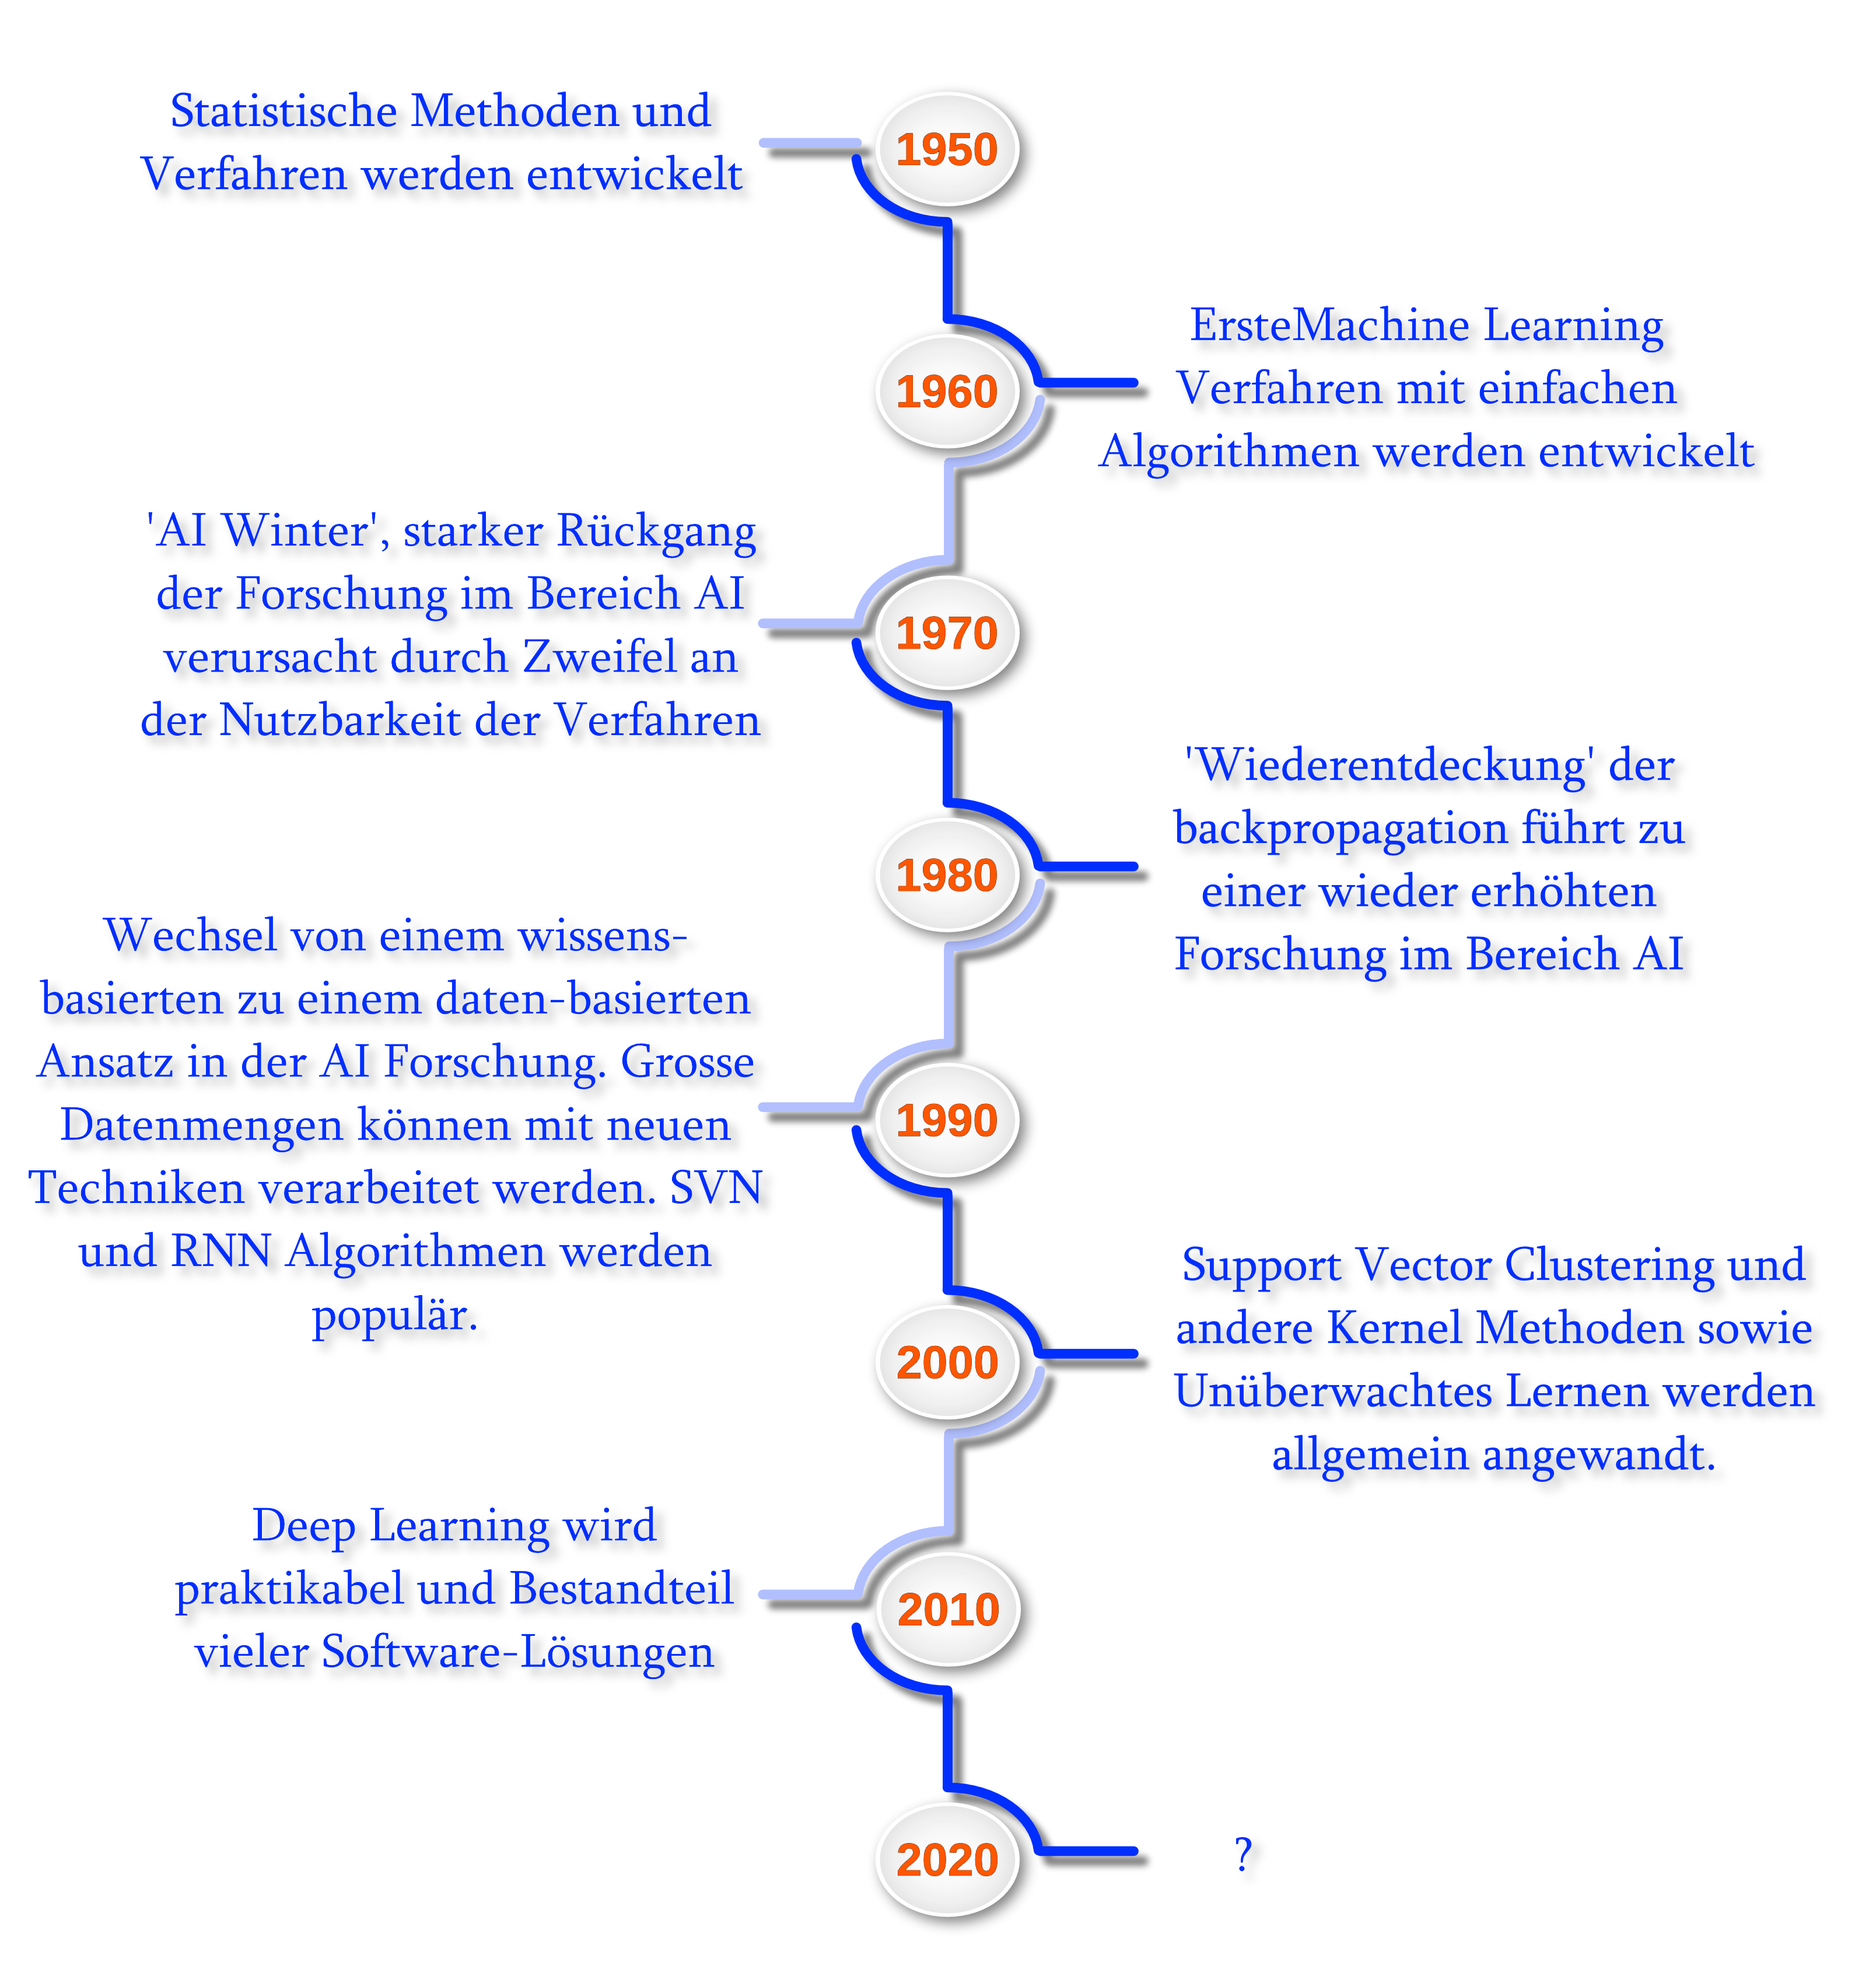
\includegraphics[width=\textwidth]{Bilder/ML-Timeline.png}
	\caption{Entwicklung des Machine Learning als Zeitachse.}
\end{figure}

Während für viele Dienste im Internet (Bildersammlungen, Empfehlungssysteme) keine oder nur geringe Anforderungen an ein verständliches Modell gestellt werden gibt es einige Bereiche in denen besondere Regeln für die Nachvollziehbarkeit von Entscheidungen bestehen.

 Exemplarisch werden hier einige dieser Gebiete aufgeführt:

\begin{description}
  \item[Medizin] \gls{ML} Anwendungen für die Krebserkennung bieten grosses Potenzial. Insbesondere die ermüdenden Aufgabe auf Röntgen- oder MRT-Bildern Spuren eines Tumors zu erkennen könnten durch \gls{ML} abgelöst werden. Allerdings sind die Zulassungskriterien für solche Lösungen noch nicht definiert.
  \item[Justiz] Predictive Policing versucht mittels statistischer und \gls{ML} Verfahren Orte oder Personengruppen zu erkennen welche  Schauplatz oder Täter/Opfer eines Verbrechens werden könnten.
  \item[Selbstfahrende Fahrzeuge] Obwohl Selbstfahrende Fahrzeuge seit Jahren von allen grossen Fahrzeugherstellern entwickelt werden sind immer noch viele Fragen bezüglich der Haftung und Zulassung offen.
\end{description}

Aufgrund des Mangels an Techniken um fortgeschrittene \gls{ML} System zu Verstehen, entstand deshalb ein neues Forschungsgebiet \acrfull{xai} welches sich zum Ziel gesetzt hat Methoden und Werkzeuge zu entwickeln um \gls{ML} Modelle zu analysieren.

\chapter{Was bedeutet Erklärbarkeit?}
\gls{ML} erzeugt Resultate welche je nach Anwendungsfall eine Entscheidung für Klasse (Pferd, Schaf, Auto), eine Zuordnung zu einer Gruppe (Premium-Kunde, Gelegenheitskäufer etc.) oder es wird ein numerischer Wert generiert (15 Grad Celsius am 3. April). 
Da sowohl die Erzeugung des Models als auch die Berechnung des Resultates automatisch erfolgt können die Schritte auf dem Weg zu dem Resultat nicht direkt nachvollzogen werden.

\begin{figure}[ht]
\centering

\includegraphics[width=\textwidth]{Bilder/Explanation-Flow.png}
\caption{Ablauf einer erklärbaren Machine Learning Anwendung}
\end{figure}

Eine \Gls{ML} Lösung beginnt mit der Beobachtung von realen Ereignissen in der Welt. Dies können die Anzahl Blätter und deren Länge einer Pflanzungsgattung oder auch Häuserpreise in Brooklyn sein. Diese Beobachtungen werden gesammelt und bilden die Daten Grundlage mit deren ein Model erzeugt werden kann. Aus diesem Model kann eine Erklärung erzeugt werden die ein Mensch verwenden kann um das Resultat zu erklären.
\section{Unterschiedliche Ziele}
Eine Anwendung welche \Gls{ML} einsetzt kann in mehrere Bereiche unterteilt werden.  Durch diese Aufteilung in verschiedene  Komponenten ergeben sich unterschiedliche Anforderungen an die Erklärbarkeit: \parencite{XAI2018}

\begin{description}
\item[Daten]
Aus der Sicht der Daten interessiert vor allem welcher Teil der Daten für das Ergebnis die Grösste Relevanz hat. Basierend auf dieser Erkenntnis kann das Datenset gezielt erweitert werden oder auch reduziert so dass ein ausgeglichenes Verhältnis erzeugt wird.

\item[Modell]
Kann man aus dem Modell Muster für eine bestimmte Kategorie ableiten? Dies kann helfen Fehlklassifizierungen von zusätzlichen Daten zu verhindern in dem überprüft wird ob das Modell die richtigen Features berücksichtigt.

\item[Vorhersage]
Erklärung weshalb ein bestimmtes Muster in den Daten zu der beobachteten Klassifizierung geführt hat. Dies ist insbesondere für Anwender/Kunden einer ML Lösung um a) das Verständnis für die Maschinelle Entscheidung zu erhöhen oder b) eine gesetzlich Vorgeschriebene Anfechtbarkeit der Entscheidung zu ermöglichen.
\end{description}

Ebenso gibt es bei den Interessengruppe unterschiedliche Anforderungen an die Erklärbarkeit einer ML Anwendung. Nach \parencite{Ras2018} werden dabei folgende Gruppierungen unterschieden:
\begin{description}
  \item[Experten]
  Diese Gruppe kann weiter unterteilt werden in
  	\begin{description}
  		\item[Forscher] Entwickelt neue Methoden und Algorithmen für das ML, verbessert bestehende Algorithmen
  		\item[Entwickler] Setzt bestehende Methodiken und Algorithmen ein um eine konkrete Aufgabenstellung zu lösen
	\end{description}
  \item[Benutzer]
  Auch bei den Benutzern gibt es verschiedene Ausprägungen
  	\begin{description}
  		\item[Eigentümer]
  		\item[Anwender]
  		\item[Person deren Daten verwendete wird]
  		\item[Anspruchsgruppe (Stakeholder)]
	\end{description}
\end{description}
Die Anforderungen an ein erklärbares Modell unterscheiden sich so stark je nach betrachtetet Komponente und der Anwendergruppe. Daraus ergibt sich dass verschiedene Techniken benötigt werden um AI Lösungen generell erklärbar zu machen.

\section{Herausforderungen durch Datenschutz}

\section{Diskriminierung}

\section{Bessere Anwendungen durch Einblick in die Funktionsweise}

\section{Weniger Angriffsflächen}

\section{Haftungsfragen}

\chapter{Anwendung von XAI auf Modelle}
Nach \parencite{Oh2019} hat Art des Modells von grossem Einfluss auf die Möglichkeiten der Erklärbarkeit. Generell wird unterschieden zwischen
\begin{description}
\item [Whitebox Modelle] sind unter der Kontrolle desjenigen welcher eine erklärende Analyse durchführt, sowohl die Daten wie der Aufbau des Modelles sind bekannt
\item[Blackbox Modelle] sind von unbekannter Struktur, der Anwender bekommt von einem gegebenen Input ein Resultat ohne den Ablauf der Entscheidungsfindung beobachten zu können
\end{description}

Aus der Vielzahl von Werkzeugen welche existieren um \acrfull{ML} Modelle zu analysieren gilt es die für den jeweiligen Use Case relevanten Werkzeuge anzuwenden.
TODO: Übersicht der Techniken und Anwendungsbereiche wie in der Grafik

\section{Anwendungsfälle}
\subsection{Exploration}
\begin{itemize}
	\item Biplot
	\item Darstellung der Korrelation (Correlation graph)
	\item Korrelationsmatrix
	\item Heatmap
	\item Parallele Koordinatendarstellung (Parallel coordinates plot)
	\item Projektion MDS, 1-SNE, UMAP
	\item Radar Plot
	\item Scatter Plot
	\item Univariate Statistiken: Häufigkeits-Verteilung, Histogram, Pivot-Tabelle
\end{itemize}
\subsection{Feature Engineering}
\subsection{Ein interpretierbares Model erstellen}
\begin{itemize}
	\item Entscheidungsbaum
	\item \acrfull{gam}
	\item \acrfull{glm}
	\item \acrfull{lfr}
	\item \acrfull{m-gbm}
	\item \acrfull{pate}	
	\item \acrfull{sbrl}
	\item \acrfull{slim}
\end{itemize}
\subsection{Modelle interpretieren}
Neben vielen Methoden welche nur für bestimmte Klassen von Verfahren anwendbar sind, gibt es einige die Allgemein anwendbar sind.

\begin{itemize}
	\item[LIME] \ref{lime}
\end{itemize}

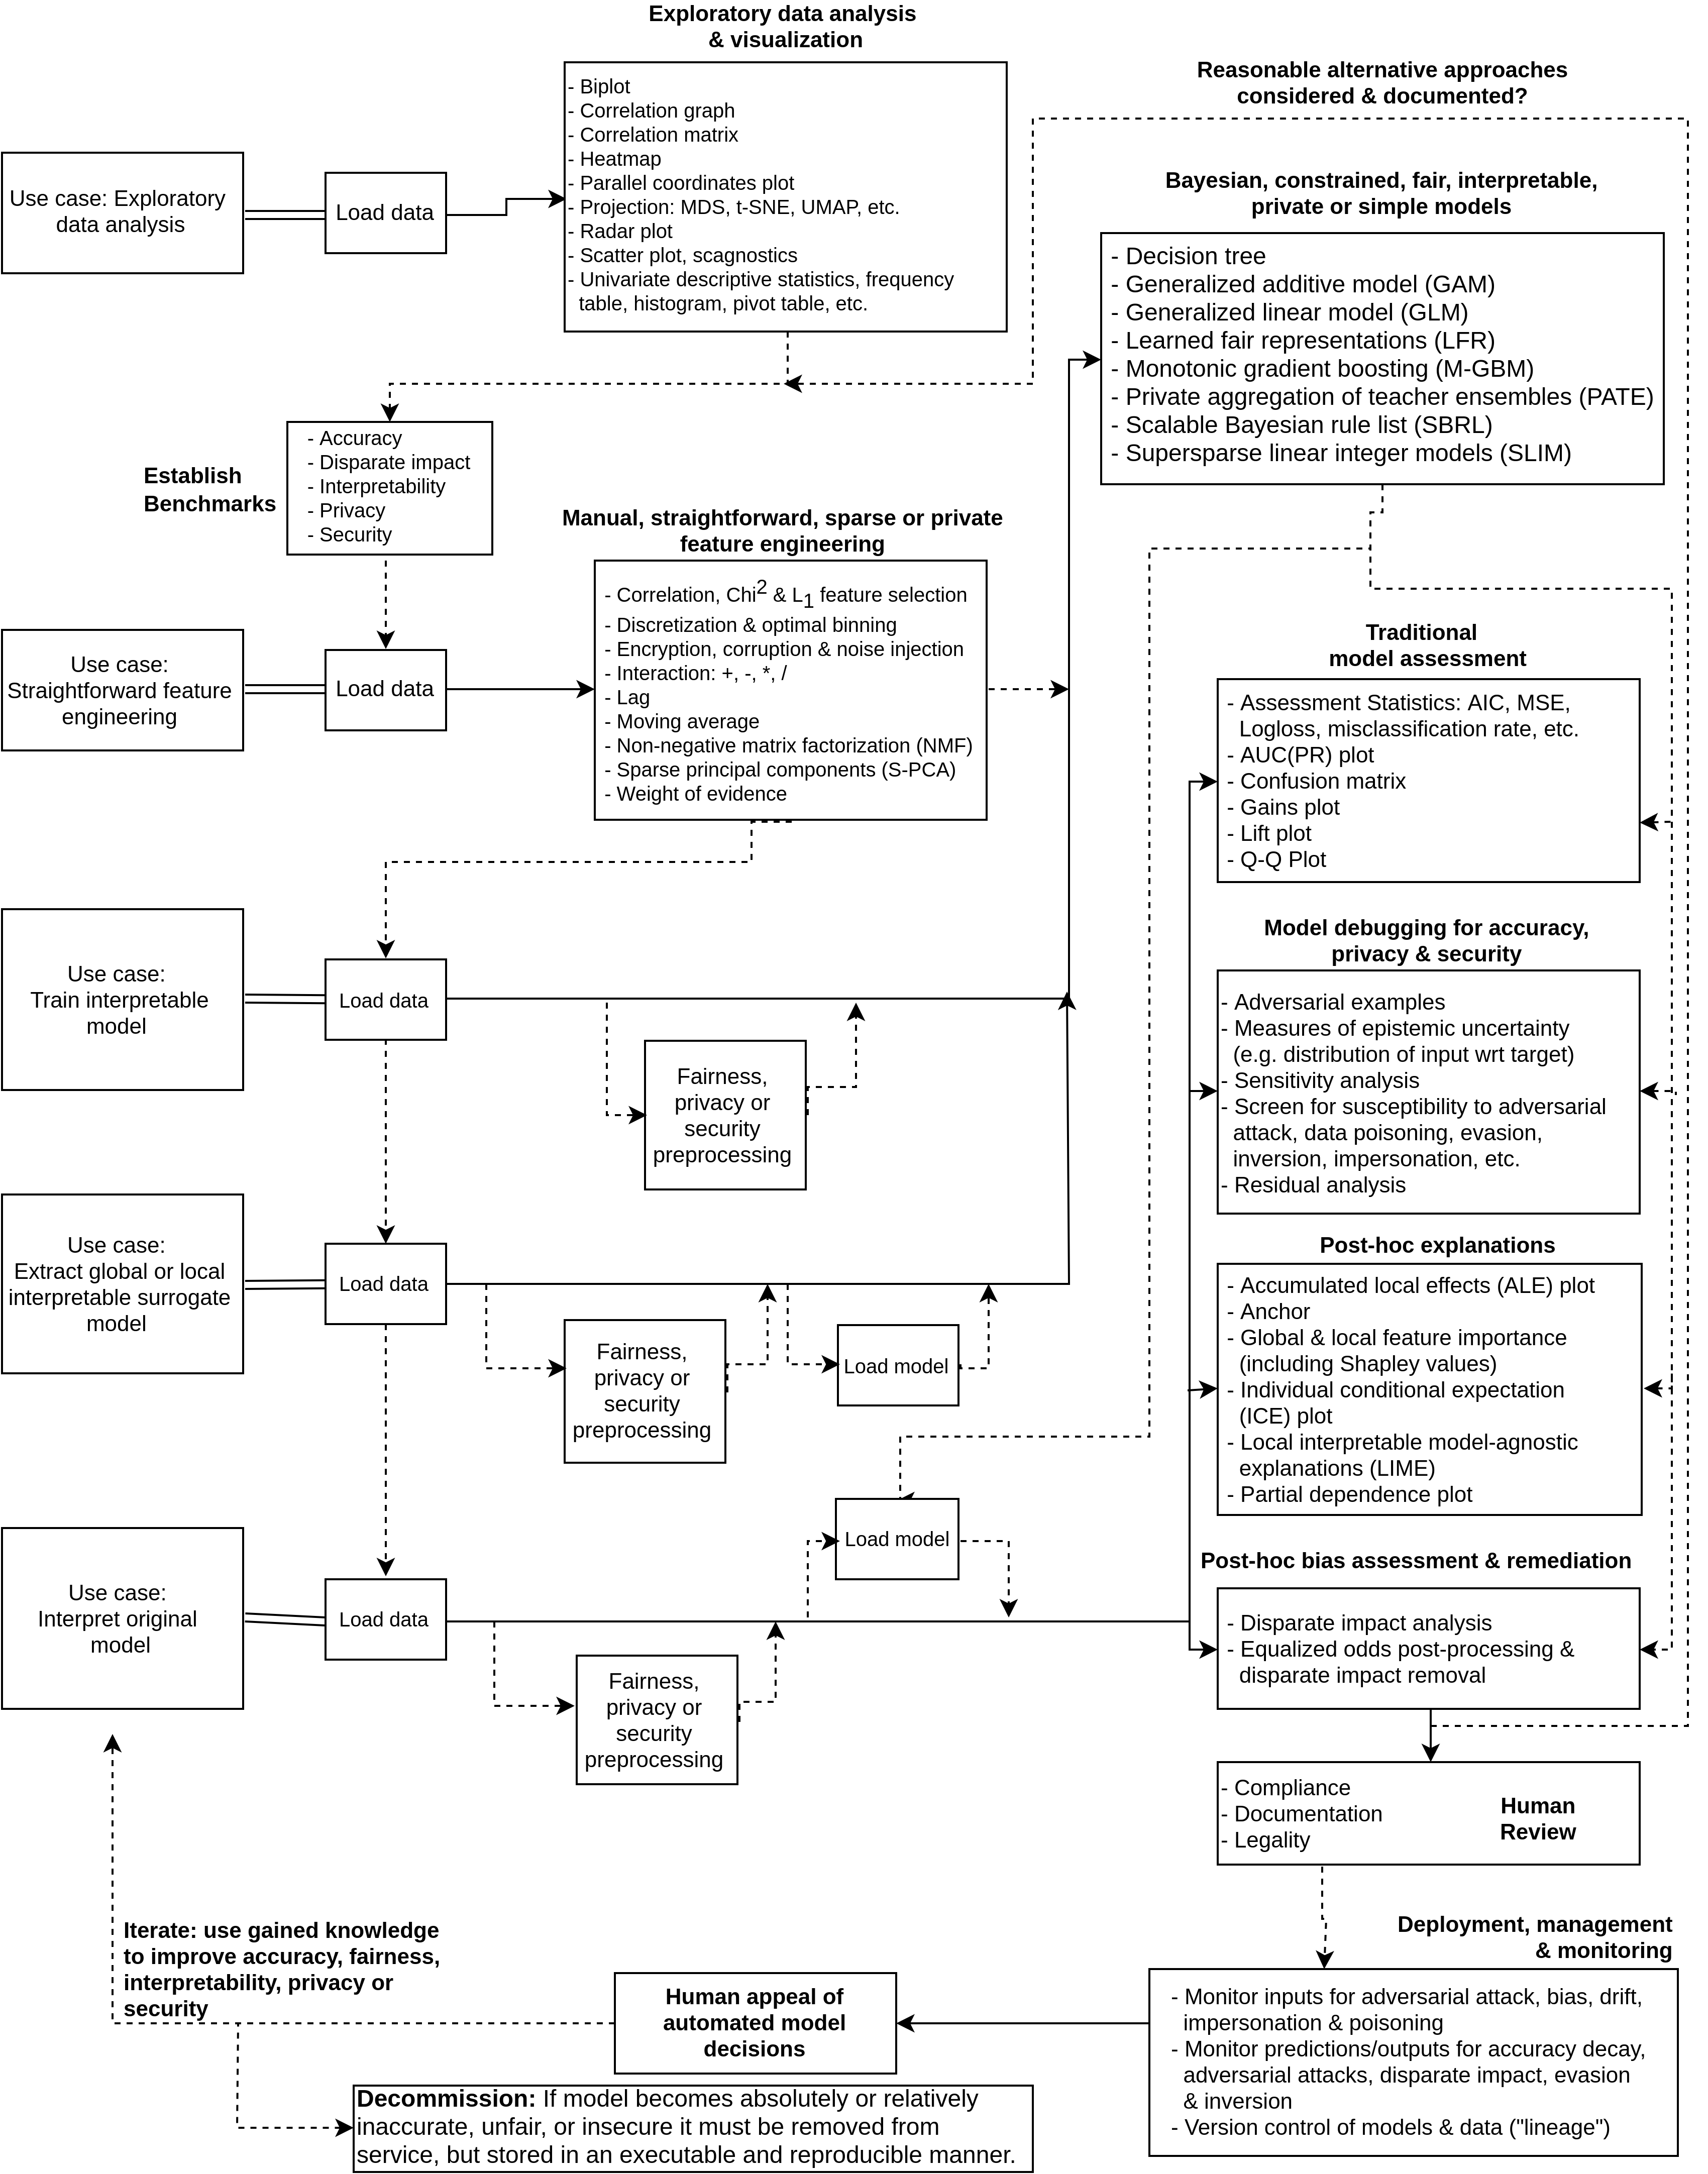
\includegraphics[width=\textwidth]{Bilder/blueprint.png}
\captionof{figure}{Quelle: https://github.com/h2oai/mli-resources}

\section{Grundsätzlich erklärbare Algorithmen}
\subsection{Lineare Regression}
Lineare Regression ist seit langer Zeit ein nützliches Werkzeug für Statistiker und Informatiker. Die Zusammenhänge zwischen dem Berechneten Ergebnis und den Eingangsvariablen können einfach nachvollzogen werden. Lineare Regression ist weit verbreitet, auch in nicht Informatik nahen Gebieten wie Medizin oder Soziologie. Ein Nachteil dieser Methode ist jedoch kleinere Leistungsfähigkeit in Bezug auf die Vorhersagequalität so dass heutzutage oftmals auf leistungsfähigere, jedoch schlechter verständliche, Algorithmen zurückgegriffen wird. Insbesondere im Gebiet der Klassifikation zeigt die Lineare Regression Schwächen.

\begin{center}
\begin{minipage}[t]{0.45\linewidth}
\vspace{0pt}
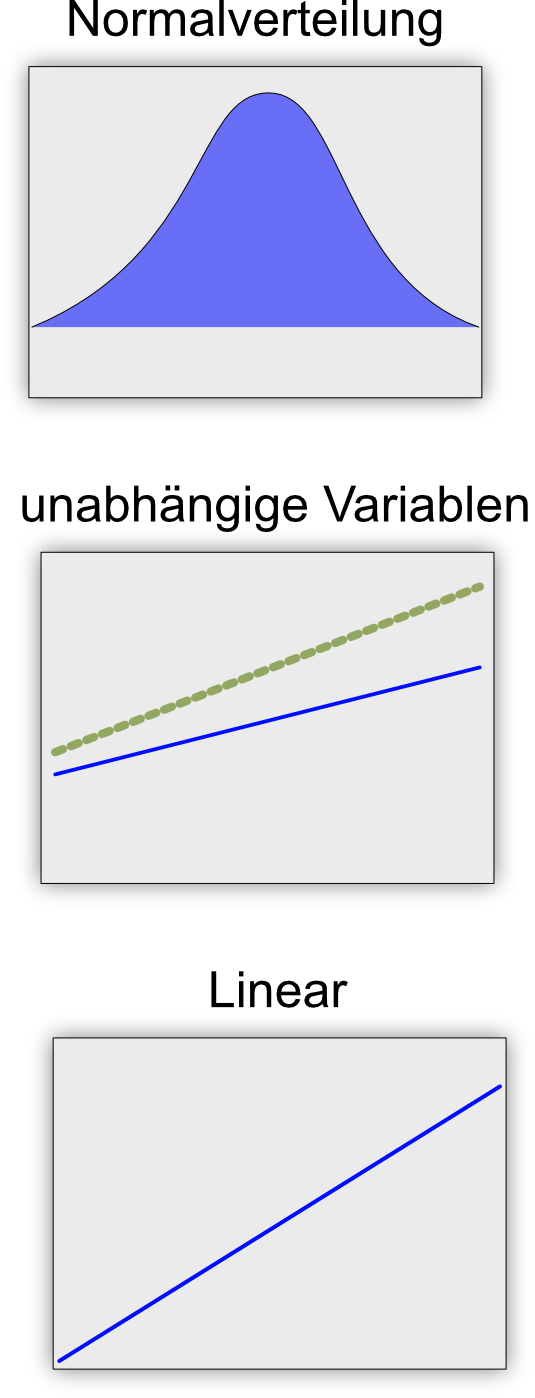
\includegraphics[width=0.6\linewidth]{Bilder/Regressions-Bedingungen.png}
 \captionof{figure}{Bedingungen lineare Regression}
\end{minipage}\hfill
\begin{minipage}[t]{0.45\linewidth}
\vspace{0pt}
Um die Lineare Regression erfolgreich anzuwenden müssen drei Bedingungen erfüllt sein:
\begin{itemize}
	\item Normalverteilte Daten
	\item Die Variablen sind unabhängig, d.h. die Werte beeinflussen sich nicht, im Gegensatz zum Beispiel bei Geschlecht und Schwangerschaft
	\item Die vorhergesagten Werte sind linear
\end{itemize}
Wenn diese Bedingungen nicht erfüllt sind kann die Lineare Regression kaum erfolgreich angewandt werden.
\end{minipage}
\end{center}

\subsection{GLM/GAM}
Lineare Regression hat einige Schwächen wie z. Bsp. die Annahme der Normalverteilung, nicht korrelierte Variablen oder auch einfach bei einem nichtlinearen Zusammenhang zwischen Eingang und dem Resultat. \acrfull{glm} und \acrfull{gam} erweitern Lineare Modelle um einen breiteren Anwendungsbereich zu ermöglichen.
\begin{center}
\begin{minipage}[t]{0.45\linewidth}
\vspace{0pt}
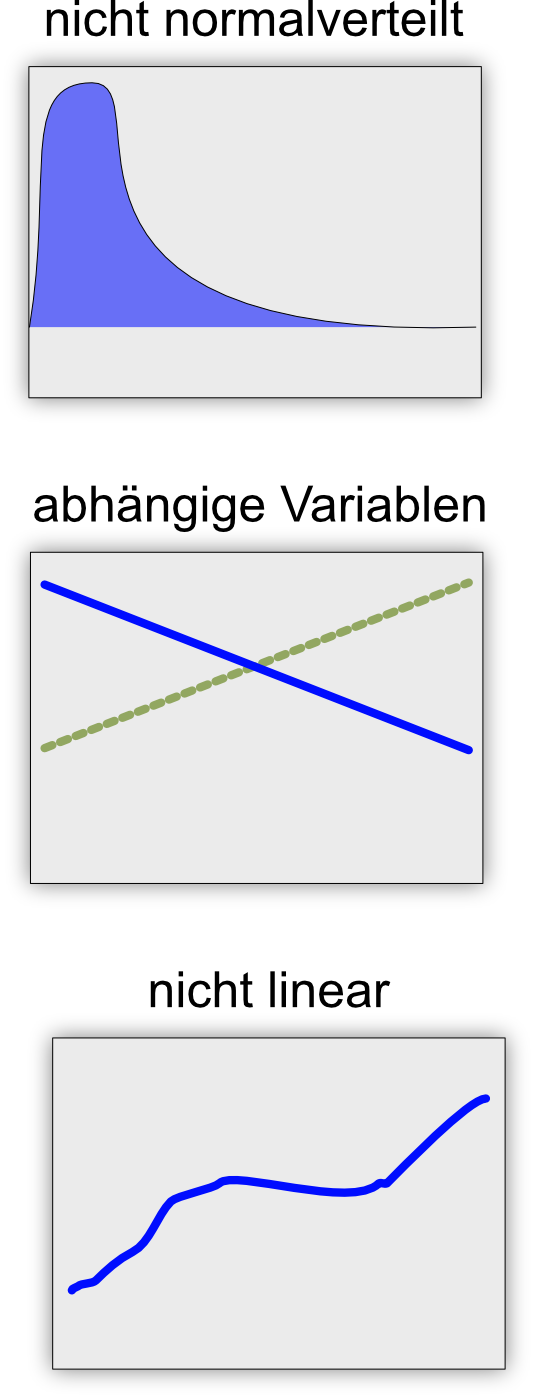
\includegraphics[width=0.6\linewidth]{Bilder/Regressions-Auschluss-Bedingungen.png}
 \captionof{figure}{Auschluss-Bedingungen lineare Regression}
\end{minipage}\hfill
\begin{minipage}[t]{0.45\linewidth}
\vspace{0pt}
Wenn die Voraussetzungen für eine Lineare Regression nicht erfüllt sind kann trotzdem mittels \Gls{glm} und \Gls{gam} eine Regression durchgeführt werden.
\end{minipage}
\end{center}

\subsection{Entscheidungsbäume}
Entscheidungsbäume (engl. Decision Tree) können bei einer geringen Anzahl von Parametern gut visualisiert werden.
\begin{center}
\begin{minipage}[t]{0.45\linewidth}
Die Regeln nach denen sich ein \Gls{DT} aufteilt können als Text dargestellt werden. Intuitiv besser verständlich sind jedoch grafische Darstellungen welche entweder den Baum als Struktur oder in einem Diagramm als Fläche darstellen.
\end{minipage}\hfill
\begin{minipage}[t]{0.45\linewidth}
\begin{lstlisting}
|--- petal width (cm) <= 0.80
|   |--- class: 0
|--- petal width (cm) >  0.80
|   |--- petal width (cm) <= 1.75
|   |   |--- class: 1
|   |--- petal width (cm) >  1.75
|   |   |--- class: 2
\end{lstlisting}
\end{minipage}
\end{center}

\begin{center}
\begin{minipage}[t]{0.45\linewidth}
\centering
	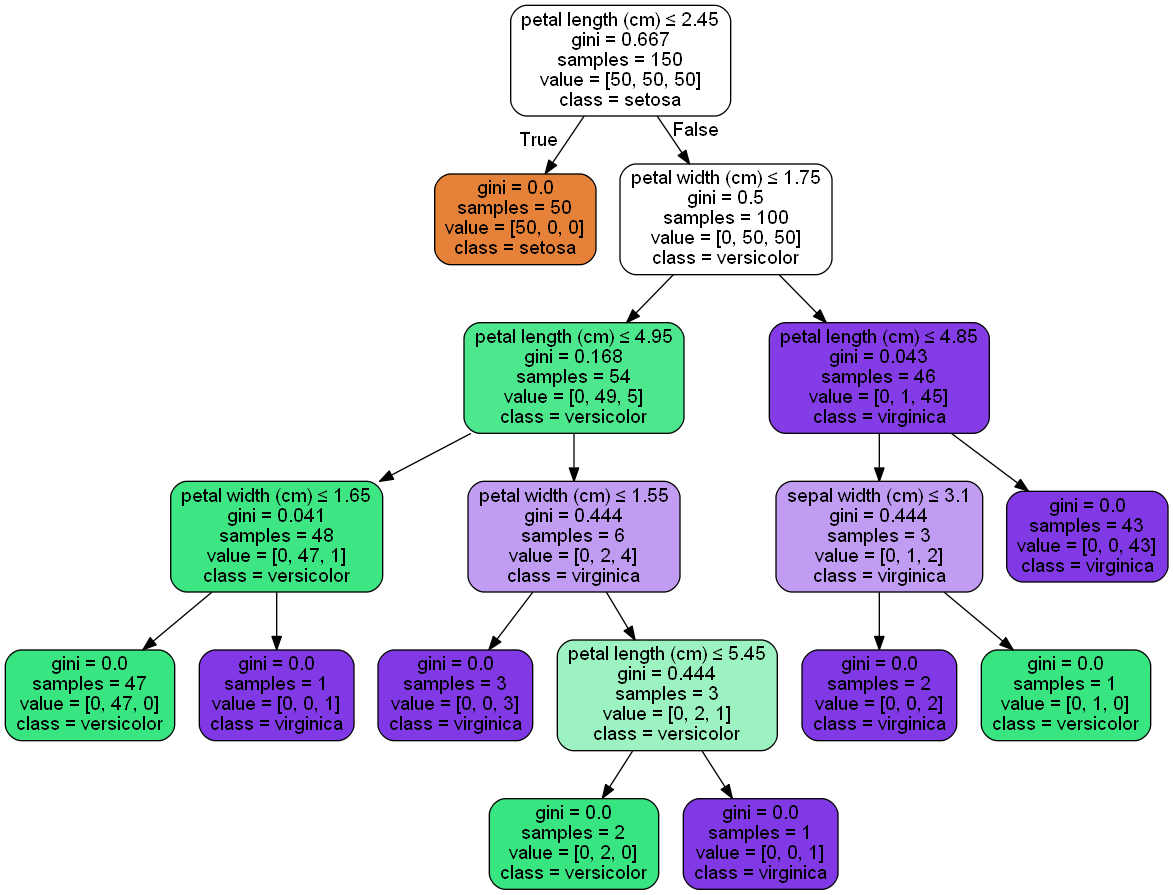
\includegraphics[width=\textwidth]{Bilder/iris-dt-explained.png}
	 \captionof{figure}{Entscheidungsbaum visualisiert.}
\end{minipage}\hfill
\begin{minipage}[t]{0.45\linewidth}
\centering
	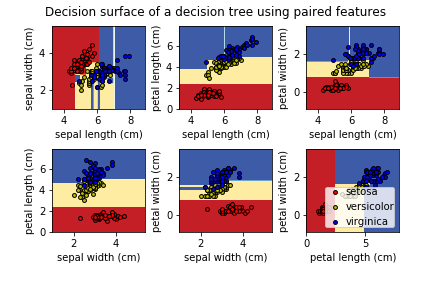
\includegraphics[width=\textwidth]{Bilder/iris-dt-decision-surface.png}
	 \captionof{figure}{Entscheidungsbaum als Flächen dargestellt}
\end{minipage}
\end{center}
Source Code \ref{dt-vis} (benötigt min. scikit-learn 0.22)

\subsection{RuleFit}
RuleFit \parencite{Friedman2008} verwendet Entscheidungsbäume um daraus Regeln abzuleiten welche neue Features erzeugen die von einem Linearen Modell verwendet werden. 
\subsection{Naive Bayes}

\section{Bilderkennung}
In den letzten Jahrzehnten wurden grosse Fortschritte in der Bilderkennung gemacht. Verantwortlich dafür sind vor allem Neuronale Netze, insbesondere die Techniken \acrfull{cnn} in Zusammenhang mit {dnn}. Neuronale Netze, insbesondere die für Bilderkennung weit verbreiteten \acrfull{dnn}, sind ohne weitere Hilfsmittel kaum zu analysieren.
Durch den starken Fokus auf Neuronale Netze bei der Bilderkennung sind für diese Technik auch einige Methoden vorhanden um das Verhalten eines Modelles  auf ein Bild darzustellen.
\subsection{Analyse Neuronaler Netze}
\subsubsection*{Eigenes Modell}
\subsubsection*{ImageNet Modell}
Das für die folgenden Analysen verwendete Modell \parencite{Simonyan2014} stammt aus der ImageNet Challenge \cite{imageNet} aus dem Jahr 2014 und ist frei verfügbar. ImageNet definiert 1001 Klassen von Objekten welche erkannt werden. Eine Klassifikation mit \cite{TensorFlow} erzeugt eine Liste mit den Wahrscheinlichkeiten für alle Klassen. Mit den \acrfull{XAI} Techniken kann für jede Klasse visualisiert werden welche Bildbereiche für diese Klassifikation relevant sind.

Mittels dem Modell VGG16 aus der Tensorflow Bibliothek \cite{vgg16} wurde folgendes Bild analysiert:
\imgText{Mira.jpg}{Original Testbild Katze}{
		\begin{tabular}{ |c|c| } 
		 \hline
		 Klasse & Wahrscheinlichkeit \\
		 \hline
		 Egyptian cat & 55.31\% \\ 
		 tabby & 8.59\% \\ 
		 tiger cat & 5.59\% \\ 
		 carton & 4.63\% \\
		 toilet tissue & 3.55\% \\
		 \hline
		\end{tabular}
		\break
		Während die ersten drei Klassen alle eine Katzenart definieren ist die vierte Klasse ``Karton'' und die Fünfte ``Toilettenpapier'' unpassend. An und für sich ist die Wahrscheinlichkeit für ``toilet tissue'' mit 3.55\% sehr klein, dennoch stellt sich die Frage weshalb dies die gegenüber den verschiedenen Katzenarten nächste Klasse ist.
}

\subsubsection*{Grad CAM} \break
\Gls{Grad CAM} ist eine Technik \parencite{Selvaraju2016} um auf der Basis von Gradienten die für eine Bildklassifikation relevanten Bereiche eines Bildes hervorzuheben. Während die relevantesten Bereiche (gelb gefärbt) um den Kopf und vor allem den Ohren der Katze sind, zeigen die Darstellungen für die unpassenden Klassen auf Bereiche des Bodens.
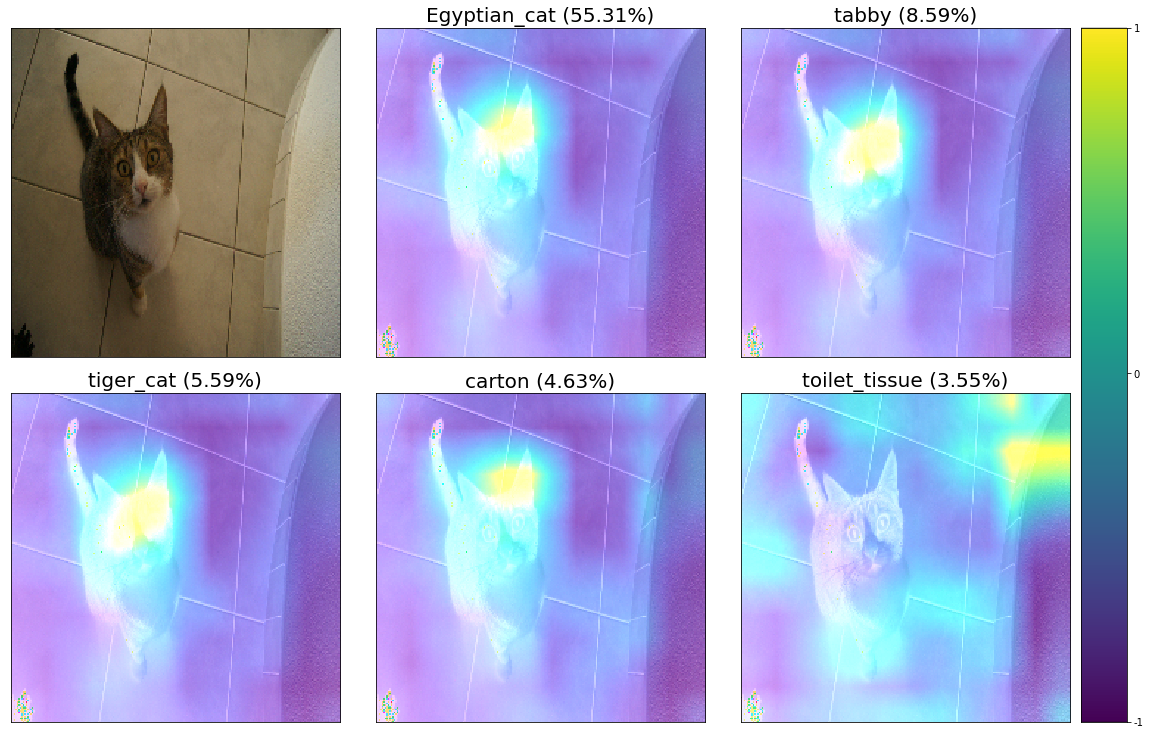
\includegraphics[width=\textwidth]{Bilder/Grad-Cam-Classes.png}

\subsubsection*{Occlusion Sensitivity} \break
Eine weitere Variante um relevante Bildbereiche aufzudecken ist Occlusion Sensitivity. Mit diesem Verfahren tritt deutlicher als bei Grad CAM die Fokusierung auf den Boden bei den beiden Falschen Klassifizierungen zutage.
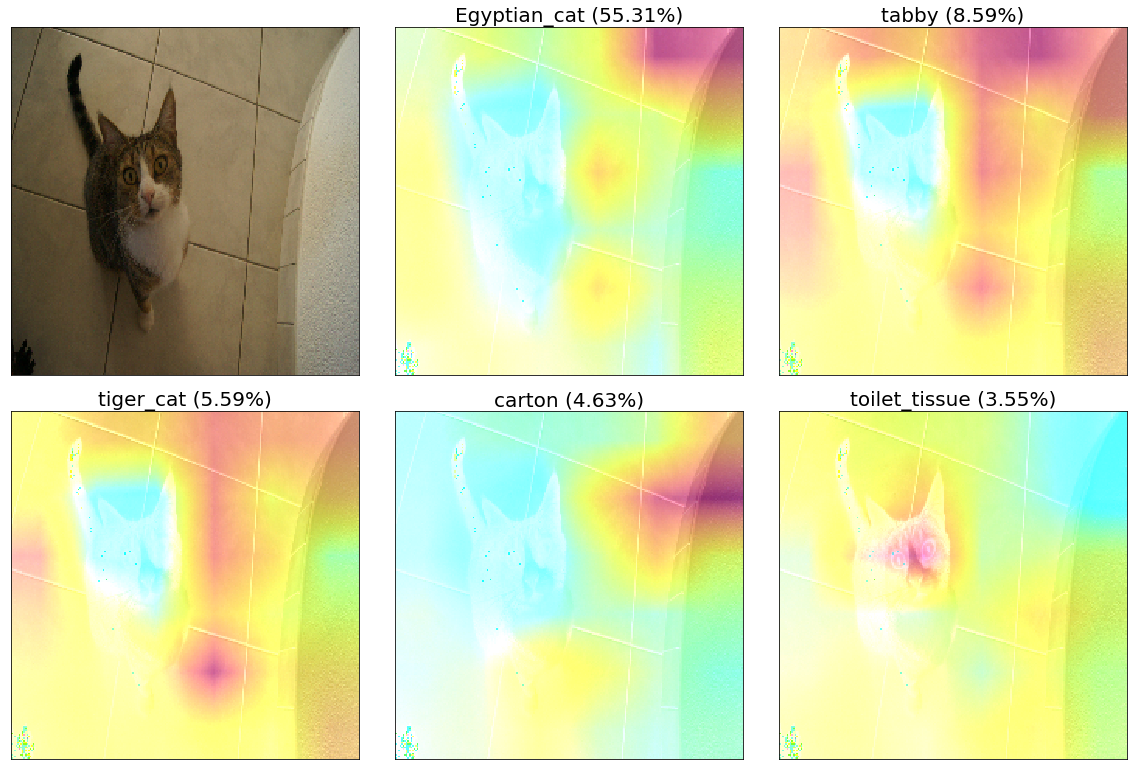
\includegraphics[width=\textwidth]{Bilder/OcclusionSensitivity-Classes.png}

\subsubsection*{LRP}
\acrfull{lrp} ist eine Technik welche ebenfalls versucht die Vorhersage eines Klassifizierers zu erklären. 

\url{ttps://github.com/VigneshSrinivasan10/interprettensor}
\url{https://github.com/sebastian-lapuschkin/lrp_toolbox}

\subsubsection*{Local Surrogate (LIME)}
\label{lime}
Die Technik LIME wurde 2016 erstmals vorgestellt \parencite{Ribeiro2016}. 
\Gls{lime} kann für verschiedene Arten von  \Gls{ML} Modellen, insbesondere auch Black Box Modelle, verwendet werden um eine Erklärung zu erzeugen. Dabei wird durch stetiges Verändern eines Eingangsbildes der Einfluss auf das Resultat geprüft. Mit den veränderten Eingangsdaten und den durch das Black Box Modell erzeugten Resultaten wird anschliessend ein neues Modell Trainiert das danach untersucht werden kann.

\paragraph*{}
Folgende Schritte werden bei der Anwendung von LIME durchgeführt:
\begin{itemize}
	\item Die Klasse für die man eine Erklärung erstellen will muss festgelegt werden
	\item Die ursprünglichen Daten werden verändert und die Resultate des Black Box Modells für diese Daten werden aufgezeichnet
	\item Die neu erzeugten Datensätzen werden nach der nähe zu der gesuchten Klasse gewichtet
	\item Ein neues Modell mit den gewichteten (neuen) Datensätzen wird erzeugt
	\item Die Vorhersage des Black Box Modells wird durch Interpretation des neu generierten Modelles erklärt
\end{itemize}
\break
In diesem Beispiel ist ersichtlich welche Bildbereiche (maskiert) nach \gls{lime} für das Resultat verantwortlich sind.

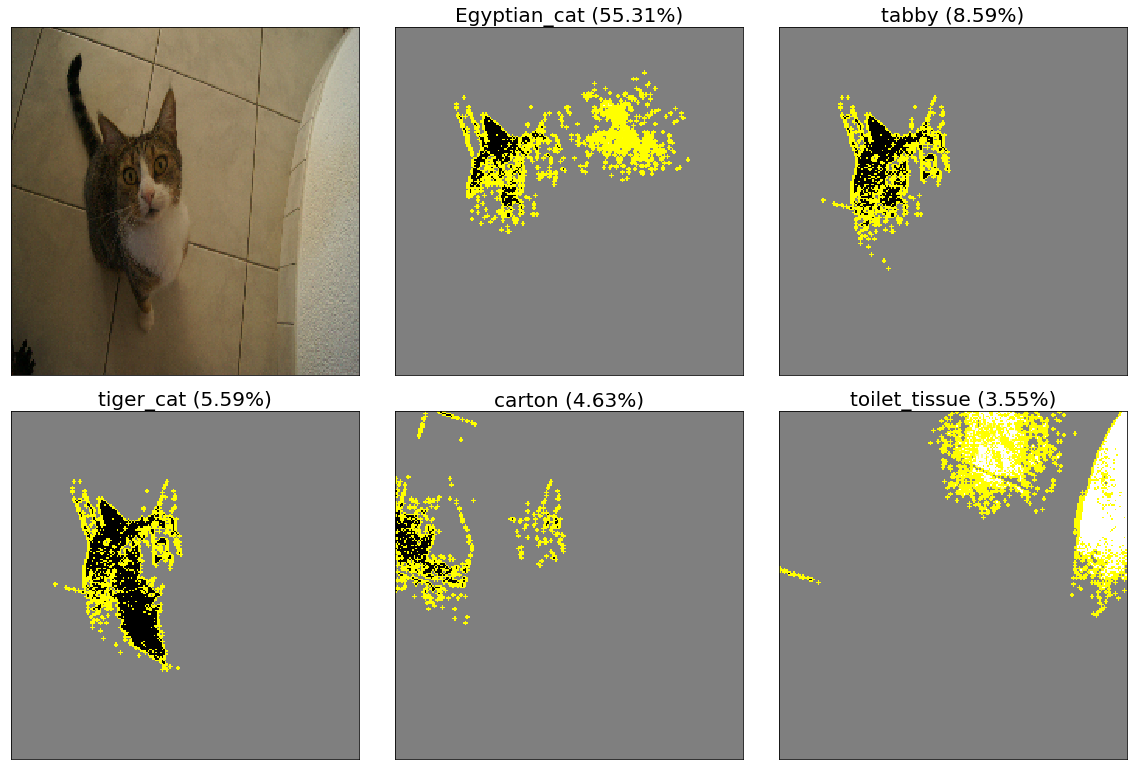
\includegraphics[width=\textwidth]{Bilder/Lime-Classes.png}
 \captionof{figure}{Darstellung relevanter Bildinhalte durch LIME}

Gegenüber den vorherigen Methoden ist LIME durch die Erzeugung temporärer Modelle bedeutend aufwendiger und dadurch auch langsamer.
\clearpage
\subsubsection*{TCAV}
 \acrfull{tcav} wurde 2017 vorgestellt \parencite{Kim2017} und ist eine fortgeschrittene Methode um Erklärungen basierend auf den Bildinhalten zu generieren. Zu diesem Zweck werden zusätzliche Modelle als Beispiele für Bildinhalte erzeugt. Ein als Zebra klassifiziertes Bild kann so zum Beispiel damit begründet werden dass auf dem Bild streifen und ein Pferd entdeckt wurden.
 \begin{figure}[ht]
\centering
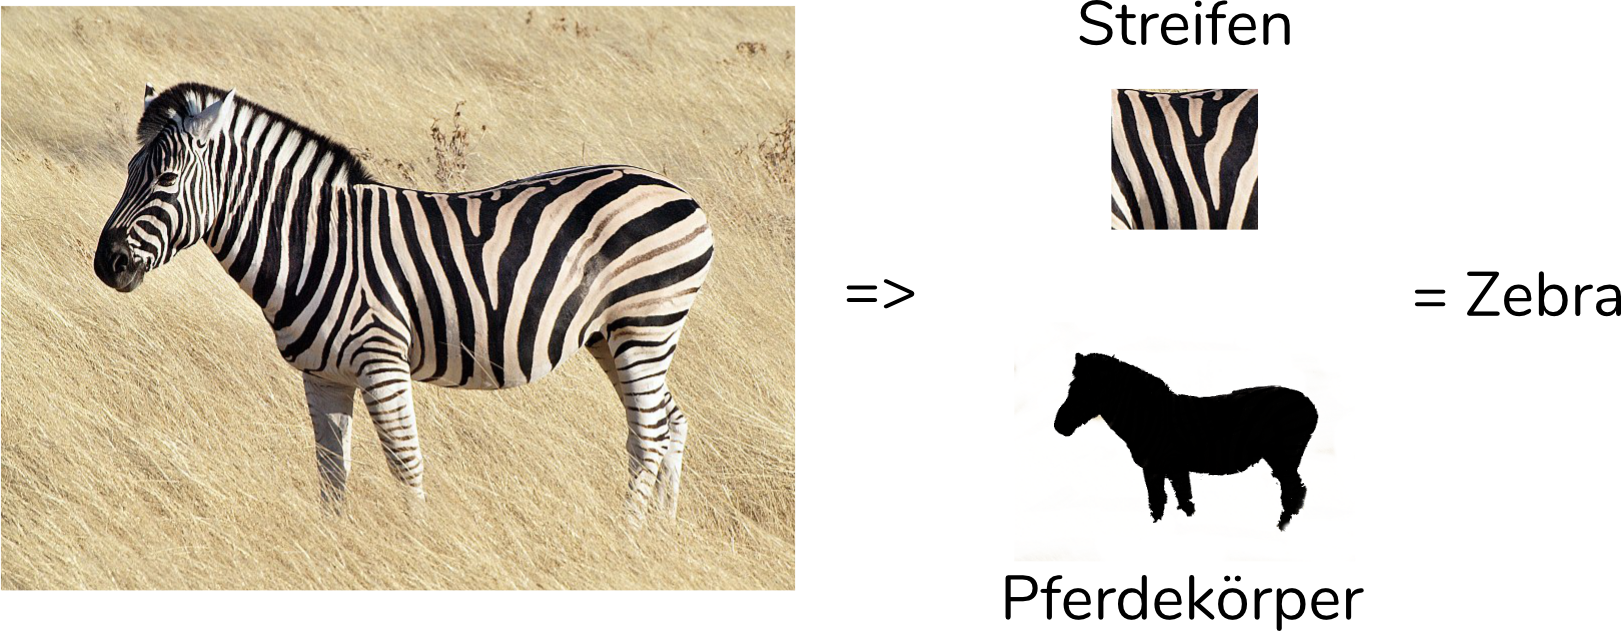
\includegraphics[width=\textwidth]{Bilder/Zebra-Explanation.PNG}
\caption{Darstellung Vorgehensweise TCAV}
\end{figure}
\url{https://github.com/tensorflow/tcav}

\subsubsection*{SVCCA}
\acrfull{svcca} vergleicht verschiedene Neuronale Netzwerke oder verschiedene Layer innerhalb des selben Neuronalen Netzwerkes.

\subsection*{Weiterführende Experimente}
Obwohl das vorhergehende Bild korrekt als Katze klassifiziert wurde, fallen die 4. und 5. Klassifikation auf. Die Klassifizierung als Karton (4.6\%) oder Toilettenpapier (3.6\%) ist zwar nicht sehr wahrscheinlich, es stellt sich aber die Frage weshalb keine weiteren Tiere welche grössere Ähnlichkeit mit einer Katze aufweisen gefunden wurden.

\subsubsection*{Anderes Tier, gleicher Hintergrund}
\imgText{IMG_2729.JPG}{Testbild Meerschweinchen}{
	\begin{tabular}{ |c|c| } 
		 \hline
		 Klasse & Wahrscheinlichkeit \\
		 \hline
		cockroach & 31.89\% \\
		Australian terrier &  8.14\% \\
		English springer & 5.48\% \\
		Irish setter & 4.95\% \\
		Blenheim spaniel & 4.74\% \\
		umbrella & 2.16\% \\
		tick & 1.57\% \\
		admiral & 1.53\% \\
		weasel  & 1.34\% \\
		centipede & 1.31\% \\
		Sussex spaniel & 1.00\% \\
		Irish water spaniel  & 0.99\% \\
		papillon & 0.99\% \\
		Welsh springer spaniel  & 0.96\% \\
		toilet tissue & 0.92\% \\
		\end{tabular}
}
\break
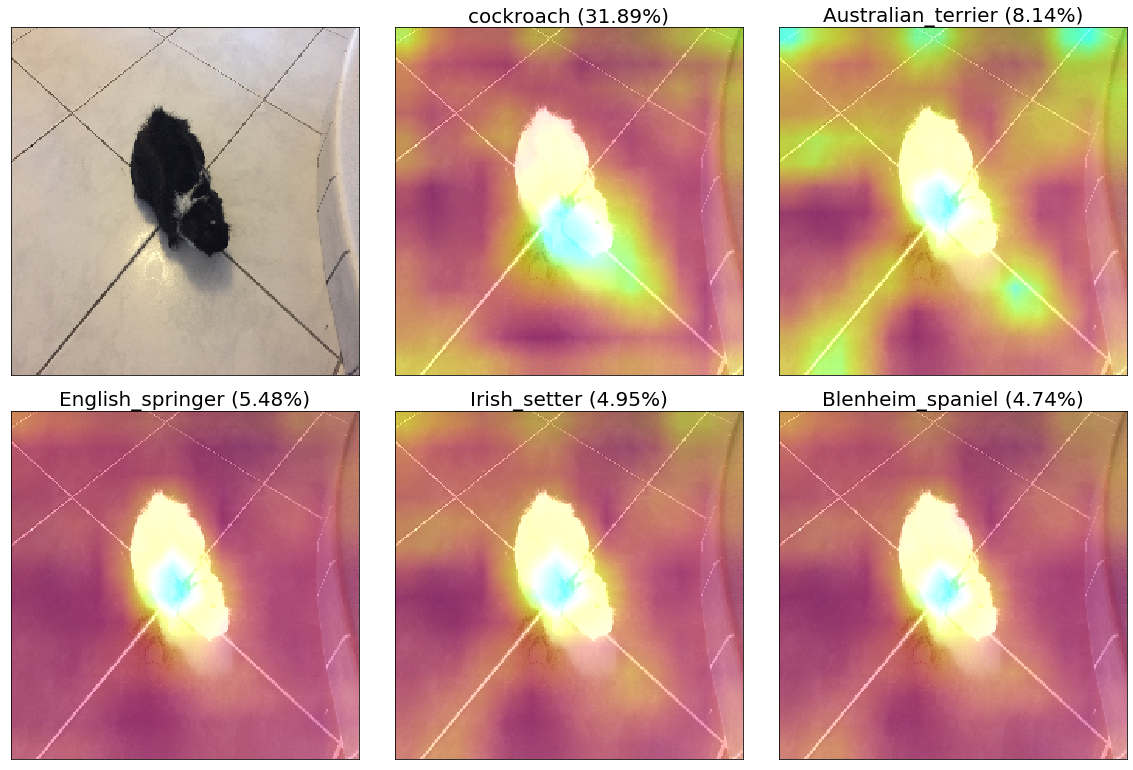
\includegraphics[width=\textwidth]{Bilder/Oreo-Grad-Cam-Classes.png}

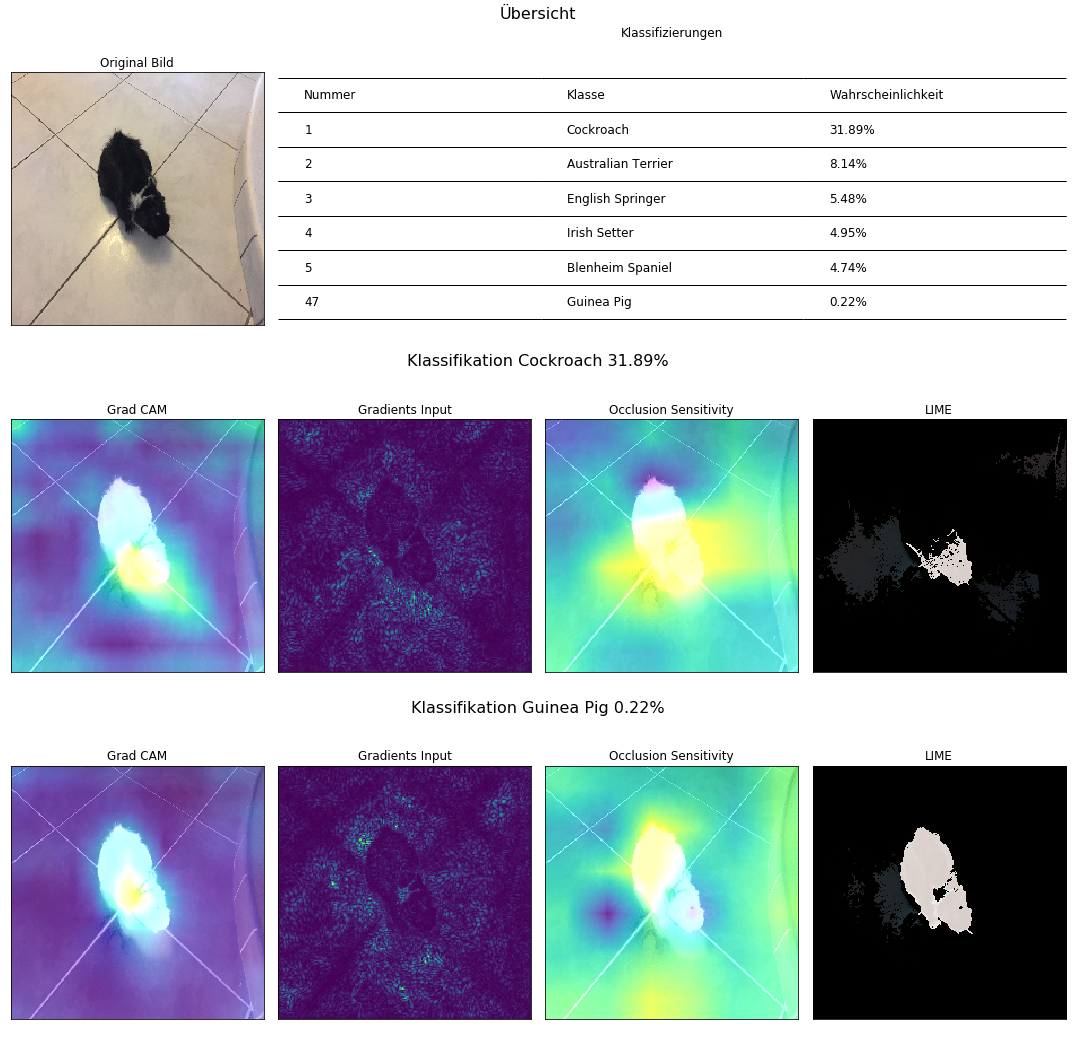
\includegraphics[width=\textwidth]{Bilder/Oreo-Classification.png}
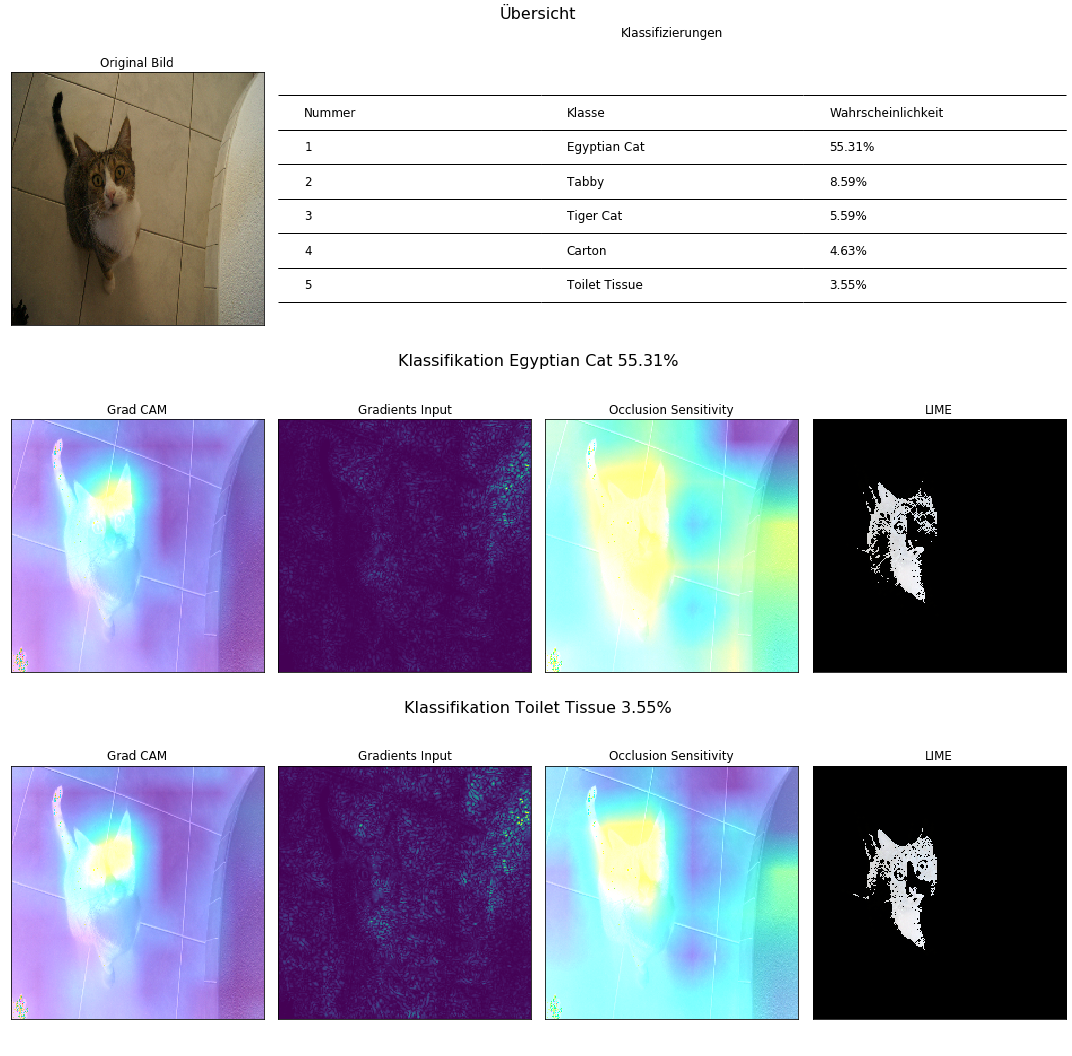
\includegraphics[width=\textwidth]{Bilder/Mira-Classification.png}
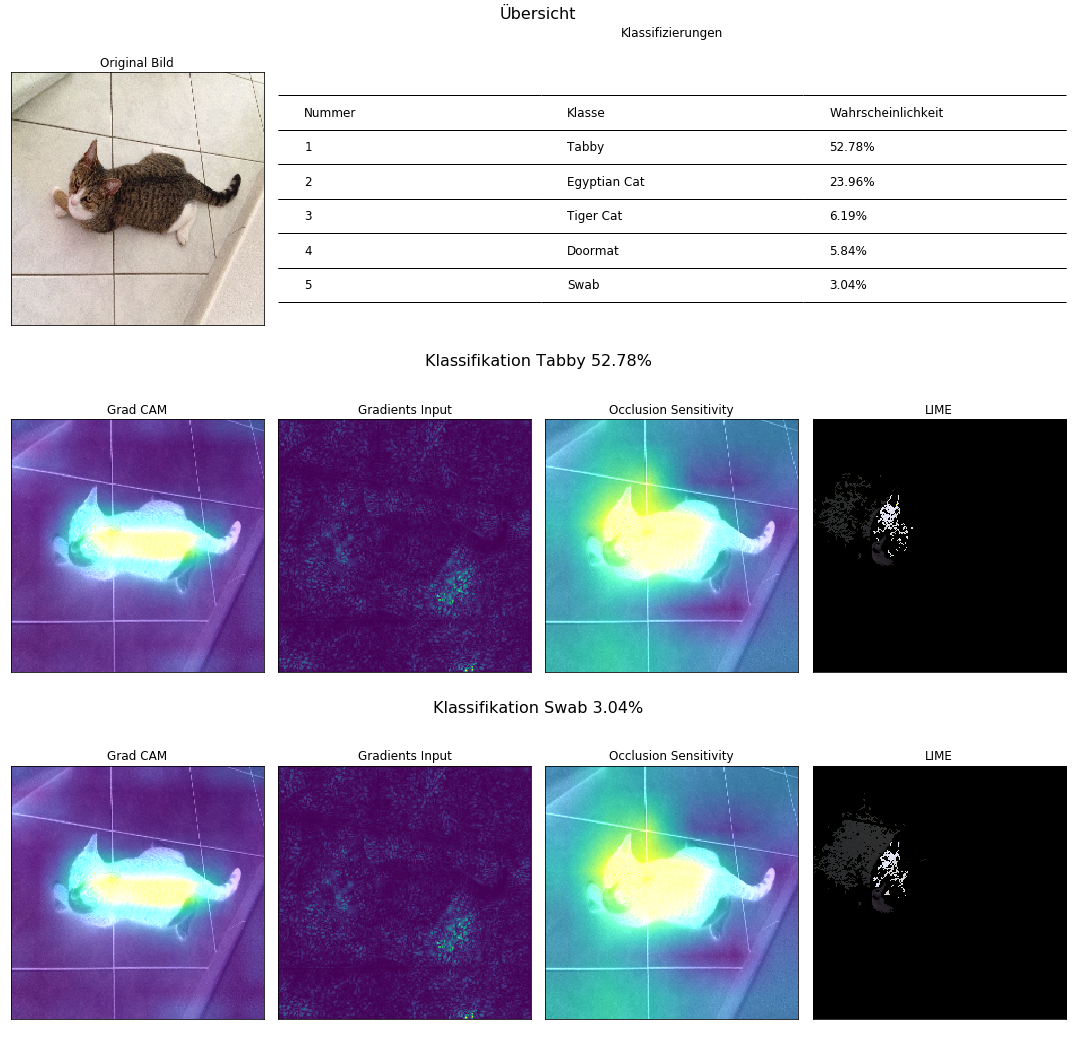
\includegraphics[width=\textwidth]{Bilder/Mira-Classification-2.png}
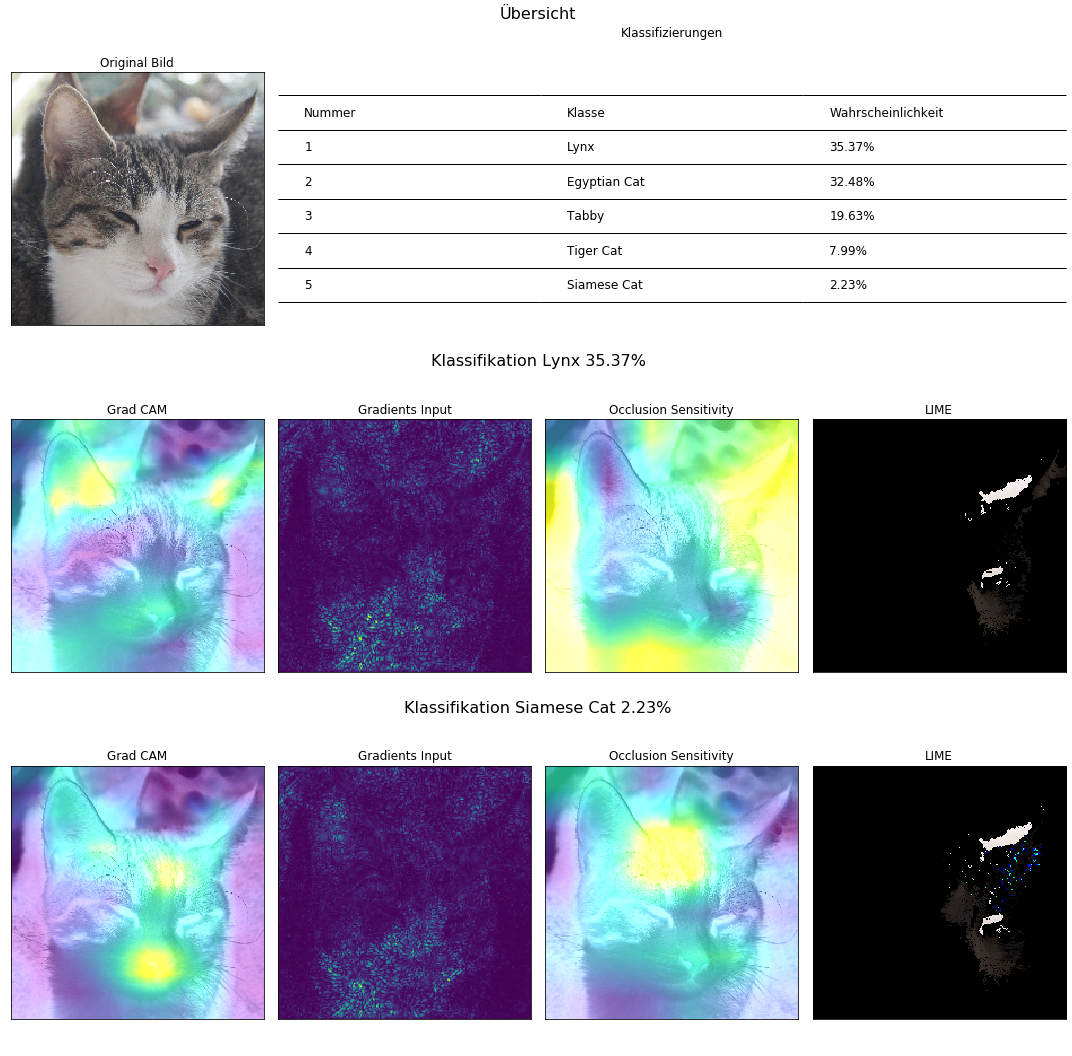
\includegraphics[width=\textwidth]{Bilder/Merlin-Classification.png}
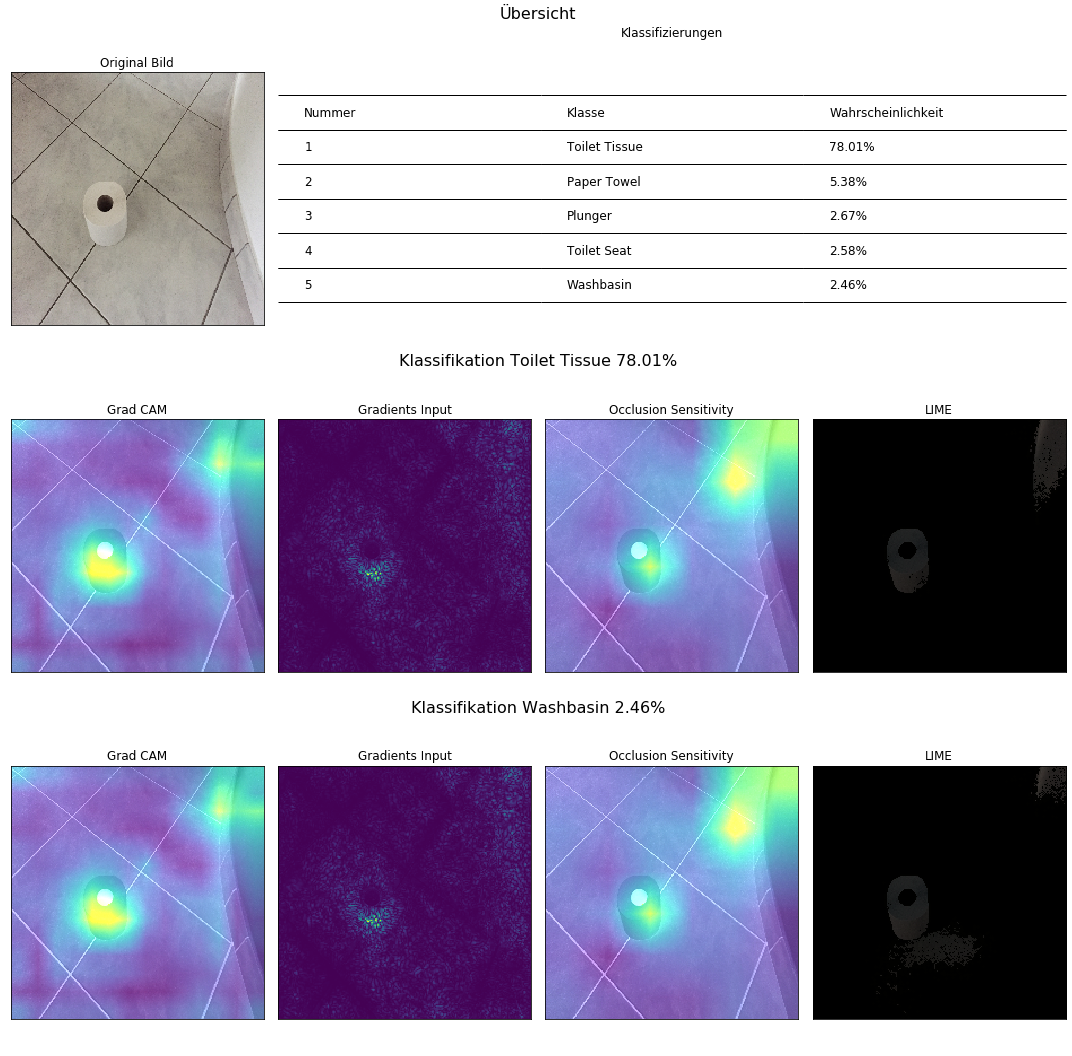
\includegraphics[width=\textwidth]{Bilder/Toilett-Tissue-Classification.png}

\section{Texterkennung}
Auch im Bereich der Texterkennung kann ein besseres Wissen über die Funktionsweise einer \Gls{ML} Anwendung sowohl den Entwicklern als auch Anwendern helfen. Insbesondere bei den Problemstellungen Sentiment Analyse und Dokumenten Klassifikation kann \Gls{XAI} das Verständnis fördern.

\subsection{Stimmungs-Analyse von Film-Bewertungen}
Das folgende Beispiel visualisiert eine Sentiment Analyse von Bewertungen von Kinofilmen. Grundlage für das Experiment ist ein Tutorial \cite{movieReview} welches generell die Text Analyse mit \cite{scikit-learn} erläutert. Die Daten stammen aus einer Arbeit von Bo Pang and Lillian Lee \parencite{Pang+Lee2004} aus dem Jahre 2004 und sind ein Auszug von Film Reviews der Internetplattform IMDB. Jeweils 100 positive und negative Reviews werden, mit einem Testanteil von 20 Prozent, von einem RandomForest trainiert.

\begin{lstlisting}[language=Python]
from sklearn.ensemble import RandomForestClassifier

classifier = RandomForestClassifier(n_estimators=1000, random_state=0)
classifier.fit(X_train, y_train)
\end{lstlisting}

\imgText{MovieReviews-SentimentClassification_ConfMatrix.PNG}{Konfusions-Matrix Texterkennungs-Experiment}{
}
Die Konfusionsmatrix mit einer für ein Experiment annehmbare Fehlerquote und einer Accuracy von 0.855.

\subsubsection*{Visualisierung durch ELI5}
Die Python Bibliothek \cite{ELI5} unterstützt einige \gls{ML} Bibliotheken und bietet die Möglichkeit Schlüsselwörter welche für eine Klassifikation relevant sind direkt in dem Ursprungstext darzustellen. 

\begin{center}
\begin{minipage}[t]{0.45\linewidth}
\vspace{0pt}
\centering
	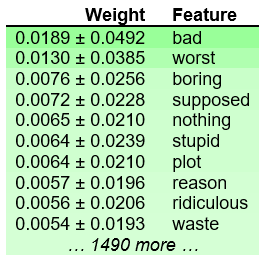
\includegraphics[width=\textwidth]{Bilder/MovieReviews-SentimentClassification_Weights.PNG}
	 \captionof{figure}{Top Features Film Review Klassifizierung}
\end{minipage}\hfill
\begin{minipage}[t]{0.45\linewidth}
\vspace{20pt}
Eine Übersicht der Top Features zeigt die Funktion ``show\_weights()''.
\begin{lstlisting}[language=Python]
eli5.show_weights(classifier, vec=vectorizer, top=10)
\end{lstlisting}
Allerdings verhält sich ELI5 bei einer binären Klassifizierung so dass nur eine Klasse (in diesem Fall `neg') dargestellt wird. Die Farbe Grün stellt immer die aktuell gewählte Klasse dar weshalb hier auch negative Wörter grün eingefärbt sind.
\end{minipage}
\end{center}

Um einen Datensatz zu visualisieren verwendete man die Methode ``explain\_prediction()'', welche sowohl Details über die Features als auch eine Darstellung des Textes mit den hervorgehobenen Schlüsselwörtern anzeigt. Je nach verwendetem Modell weicht die Darstellung von dem hier dargestellten Bild ab, bei gewissen Tree Algorithmen (z.Bsp. DecisionTree) wird zusätzlich noch die Baumstruktur angezeigt.
\begin{lstlisting}[language=Python]
doc = documents[414]
eli5.explain_prediction(classifier, doc, vec=vectorizer,target_names=['neg','pos'], top=20)
\end{lstlisting}
\begin{figure}[ht]
\centering
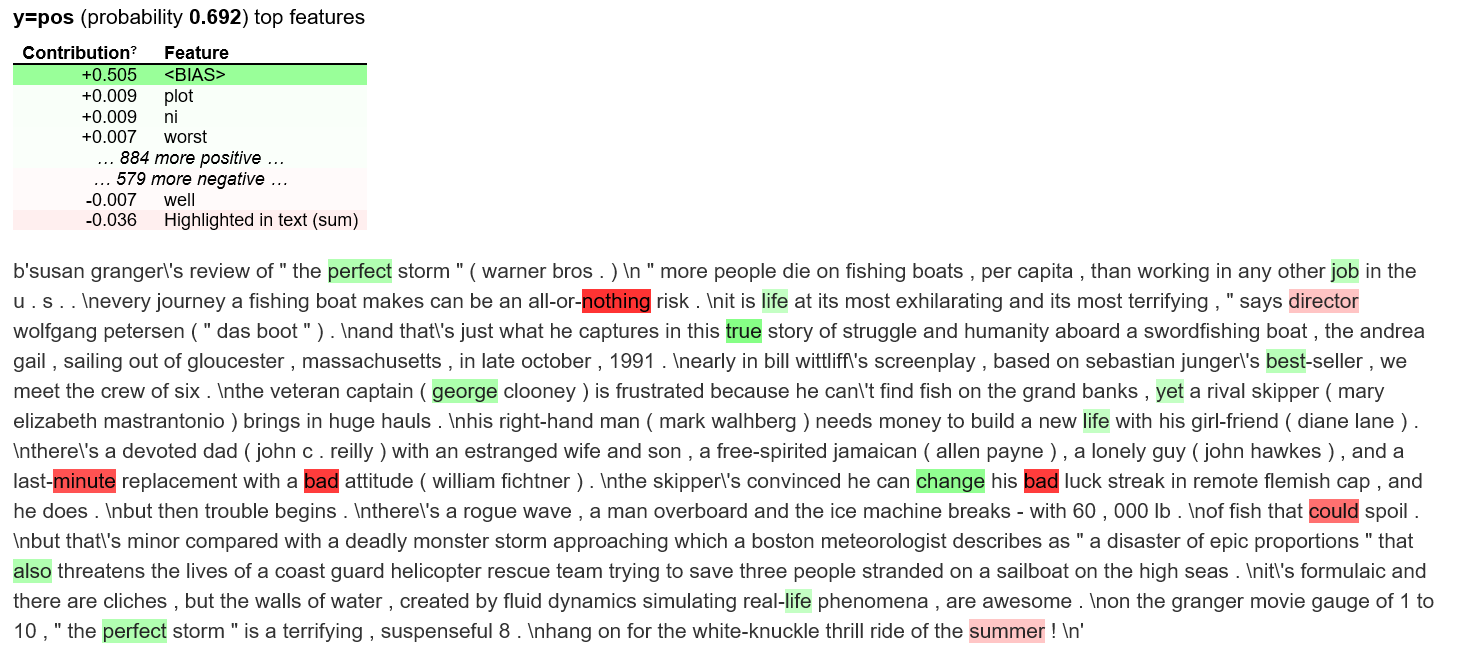
\includegraphics[width=\textwidth]{Bilder/MovieReviews-SentimentClassification_1.PNG}
\caption{Visualisierung positives Film Review}
\end{figure}

Bei der Darstellung des negativen Film Reviews fällt auf dass Wörter welche für eine negative Stimmung stehen Grün markiert sind. Dies kommt daher dass für ELI5 die wahrscheinlichste Klasse `neg' ist (81\%) und deshalb alle Schlüsselwörter welche auf diese Klasse hinweisen grün markiert werden.
\begin{figure}[ht]
\centering
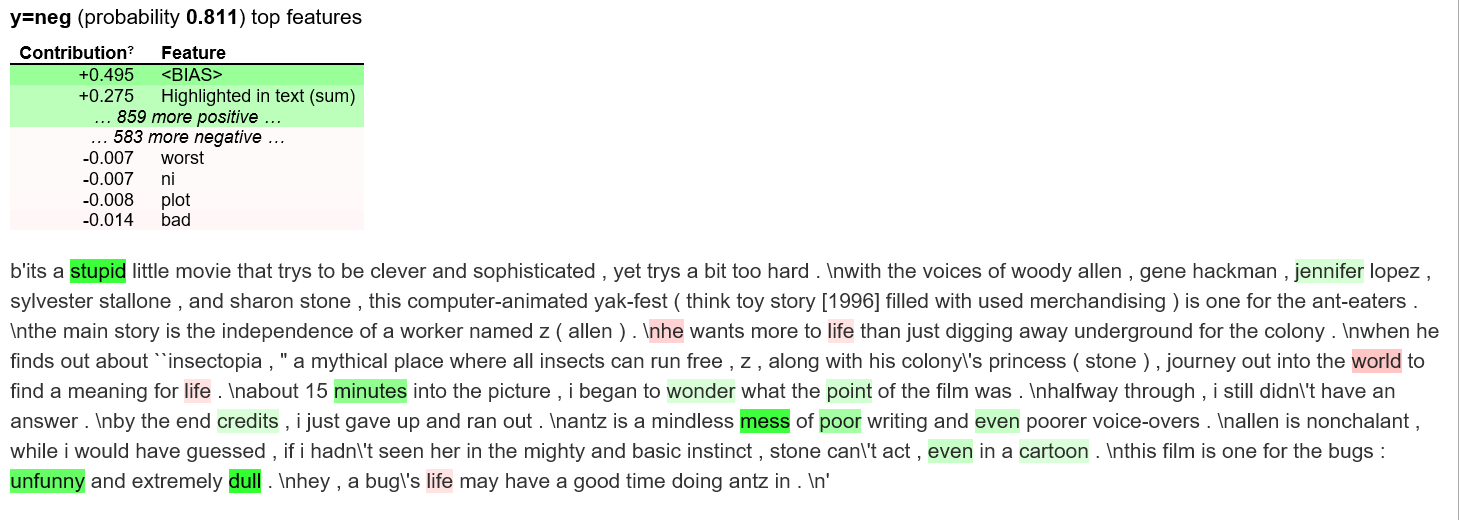
\includegraphics[width=\textwidth]{Bilder/MovieReviews-SentimentClassification_2.PNG}
\caption{Visualisierung negatives Film Review}
\end{figure}

\subsubsection*{Blackbox Visualisierung mit ELI5}
Während in dem letzten Beispiel ein White Box Model angewendet wurde, kann \cite{ELI5} auch Black Box Modelle analysieren. Dazu verwendet \cite{ELI5} eine \Gls{lime} implementation und die Vorhersage zu erklären.

\chapter{Schwächen von ML Modellen erkennen}
\section{Diskriminierung durch Bias}
\section{Adversarial Attacks}
\section{Data Poisoning}

\chapter{Weiterentwicklung von XAI}

\chapter{Anhang}
\section{Source Code}
\label{dt-vis}

\subsection{Entscheidungsbaum Visualisierung mit sklearn und Graphviz}
\begin{lstlisting}[language=Python, caption=Decision Tree Visualisierung]
from sklearn.datasets import load_iris
from sklearn import tree
from sklearn import datasets

X, y = load_iris(return_X_y=True)
clf = tree.DecisionTreeClassifier()
clf = clf.fit(X, y)

iris = datasets.load_iris()

dot_data = tree.export_graphviz(clf, out_file=None, 
                      feature_names=iris.feature_names,  
                      class_names=iris.target_names,  
                      filled=True, rounded=True,  
                      special_characters=True)  

# print tree as text
from sklearn.tree import export_text
r = export_text(clf, feature_names=iris['feature_names'])
print(r)

# print tree as colored top-down tree
import graphviz
graph = graphviz.Source(dot_data)  
graph 

# plot decision surface
import numpy as np
import matplotlib.pyplot as plt
# Parameters
n_classes = 3
plot_colors = "ryb"
plot_step = 0.02

for pairidx, pair in enumerate([[0, 1], [0, 2], [0, 3],
                                [1, 2], [1, 3], [2, 3]]):
    # We only take the two corresponding features
    X = iris.data[:, pair]
    y = iris.target
    
    # Train
    dTree = tree.DecisionTreeClassifier().fit(X, y)

    # Plot the decision boundary
    plt.subplot(2, 3, pairidx + 1)

    x_min, x_max = X[:, 0].min() - 1, X[:, 0].max() + 1
    y_min, y_max = X[:, 1].min() - 1, X[:, 1].max() + 1
    xx, yy = np.meshgrid(np.arange(x_min, x_max, plot_step),
                         np.arange(y_min, y_max, plot_step))
    plt.tight_layout(h_pad=0.5, w_pad=0.5, pad=2.5)

    Z = dTree.predict(np.c_[xx.ravel(), yy.ravel()])
    Z = Z.reshape(xx.shape)
    cs = plt.contourf(xx, yy, Z, cmap=plt.cm.RdYlBu)

    plt.xlabel(iris.feature_names[pair[0]])
    plt.ylabel(iris.feature_names[pair[1]])

    # Plot the training points
    for i, color in zip(range(n_classes), plot_colors):
        idx = np.where(y == i)
        plt.scatter(X[idx, 0], X[idx, 1], c=color, label=iris.target_names[i],
                    cmap=plt.cm.RdYlBu, edgecolor='black', s=15)

plt.suptitle("Decision surface of a decision tree using paired features")
plt.legend(loc='lower right', borderpad=0, handletextpad=0)
plt.axis("tight")
\end{lstlisting}
https://scikit-learn.org/stable/modules/tree.html

\subsection{Bild-Klassifikation mit tf-explain}
Das folgende Programm erzeugt mit den Bibliotheken Tensorflow (2.0) und tf-explain und en Algorithmen ``Grad CAM'' und ``Integrated Gradients'' Visualisierungen einer Bild-Klassifizierung. 
\begin{lstlisting}[language=Python, caption=Visualisiertes Neuronales Netz mit Tensorflow und tf-explain]
import tensorflow as tf
from keras.applications.vgg16 import VGG16
from keras.preprocessing.image import load_img
from keras.preprocessing.image import img_to_array
from keras.applications.vgg16 import preprocess_input
from keras.applications.vgg16 import decode_predictions

model = tf.keras.applications.vgg16.VGG16(weights="imagenet", include_top=True)

#print(model.summary())

imageOrig = load_img('D:/Master Thesis/dogs-vs-cats/test/DSC05797.JPG', target_size=(224, 224))
imageArr = img_to_array(imageOrig)  #output Numpy-array

imageReshaped = imageArr.reshape((1, imageArr.shape[0], imageArr.shape[1], imageArr.shape[2]))

image = preprocess_input(imageReshaped)
predictions = model.predict(imageReshaped)

import numpy as np
top5predictions = np.argsort(predictions)[0,::-1][:5]

labels = decode_predictions(predictions)

for label in labels[0]:
    print('%s (%.2f%%)' % (label[1], label[2]*100))
    
from tf_explain.core.grad_cam import GradCAM
from mpl_toolkits.axes_grid1 import ImageGrid

def createImageGrid(imageOrig, predictions, labels, explainer, explainerArgs):
    camImages = [imageOrig]
    fig = plt.figure(figsize=(20., 20.))
    grid = ImageGrid(fig, 111,  # similar to subplot(111)
                 nrows_ncols=(2, 3),
                 axes_pad=0.5,  # pad between axes in inch.
                 )
    for class_index in top5predictions:
        camImages.append(explainer.explain(class_index=class_index, **explainerArgs))
    
    i = -1
    for ax, im in zip(grid, camImages):
        # Iterating over the grid returns the Axes.
        ax.set_xticks([])
        ax.set_yticks([])
        label = labels[0][i]
        if i >= 0:
            ax.set_title('%s (%.2f%%)' % (label[1], label[2]*100), fontsize=20)
        ax.imshow(im)
        i = i + 1

    plt.show()


explainer = GradCAM()
createImageGrid(imageOrig, predictions, labels, explainer, {'model': model, 'layer_name': 'block5_conv3', 'validation_data': data})

from tf_explain.core.gradients_inputs import GradientsInputs
explainer = GradientsInputs()
createImageGrid(imageOrig, predictions, labels, explainer, {'model': model, 'validation_data': (np.array([imageArr]), None)})

from tf_explain.core.integrated_gradients import IntegratedGradients

explainer = IntegratedGradients()
createImageGrid(imageOrig, predictions, labels, explainer, {'model': model, 'validation_data': (np.array([imageArr]), None)})
\end{lstlisting}
https://github.com/sicara/tf-explain

\subsection{Visualisierung einer Klassifikation mit lime}
\url{https://github.com/marcotcr/lime/blob/master/doc/notebooks/Tutorial\%20-\%20Image\%20Classification\%20Keras.ipynb}
\begin{lstlisting}[language=Python, caption=Visualisiertes Neuronales Netz mit Tensorflow und lime]
import lime 
from lime import lime_image

explainer = lime_image.LimeImageExplainer()


explanation = explainer.explain_instance(np.vstack([imageArr]), model.predict, top_labels=5, hide_color=0, num_samples=1000)

from skimage.segmentation import mark_boundaries

camImages = [imageOrig]
fig = plt.figure(figsize=(20., 20.))
grid = ImageGrid(fig, 111,  # similar to subplot(111)
             nrows_ncols=(2, 3),
             axes_pad=0.5,  # pad between axes in inch.
             )
for class_index in range(0,5):
    temp, mask = explanation.get_image_and_mask(explanation.top_labels[class_index], positive_only=True, num_features=5, hide_rest=True)
    camImages.append(mark_boundaries(temp / 2 + 0.5, mask))

i = -1
for ax, im in zip(grid, camImages):
    # Iterating over the grid returns the Axes.
    ax.set_xticks([])
    ax.set_yticks([])
    label = labels[0][i]
    if i >= 0:
        ax.set_title('%s (%.2f%%)' % (label[1], label[2]*100))
    ax.imshow(im)
    i = i + 1

plt.show()
\end{lstlisting}
\appendix
% List of Figures
\listoffigures
% List of Tables
\begingroup
\let\clearpage\relax
\listoftables
% Glossary
\printglossary[type=\acronymtype]
\printglossary[type=main]
% Bibliography
\printbibliography

\renewcommand\bibname{Linkverzeichnis}
\begin{thebibliography}{99}\label{links}
   \bibitem{vgg16} VGG16: Modell für Imagenet Klassifikationen \break \url{https://github.com/tensorflow/tensorflow/blob/r1.8/tensorflow/python/keras/_impl/keras/applications/vgg16.py}
   \bibitem{imageNet} ImageNet Challenge \break \url{http://www.image-net.org/challenges/LSVRC/}
   \bibitem{iML}Interpretable Machine Learning, A Guide for Making Black Box Models Explainable \break \url{https://christophm.github.io/interpretable-ml-book/rulefit.html}
   \bibitem{ELI5} ELI5 Python Bibliothek um \Gls{ML} Modelle zu erklären und analysieren\break \url{https://eli5.readthedocs.io/}
  \bibitem{SVCCA}  \break \url{https://ai.googleblog.com/2017/11/interpreting-deep-neural-networks-with.html}
  \bibitem{movieReview} Beispiel einer Textanalyse mit Scikit-Learn \break \url{https://stackabuse.com/text-classification-with-python-and-scikit-learn/}
  \bibitem{scikit-learn} Scikit-Learn, \Gls{ML} Framework \break \url{https://scikit-learn.org/stable/index.html}
\end{thebibliography}
%Index
\addcontentsline{toc}{chapter}{Index}
%\printindex
% Appendices
\lstlistoflistings
\endgroup

\end{document}
